\documentclass[12pt]{ucsddissertation}
% mathptmx is a Times Roman look-alike (don't use the times package)
% It isn't clear if Times is required. The OGS manual lists several
% "standard fonts" but never says they need to be used.
\usepackage{mathptmx}
\usepackage[NoDate]{currvita}
\usepackage{array}
\usepackage{tabularx}
\usepackage{booktabs}
\usepackage{ragged2e}
\usepackage{microtype}
\usepackage[breaklinks=true,pdfborder={0 0 0}]{hyperref}
\usepackage{graphicx}
\AtBeginDocument{%
	\settowidth\cvlabelwidth{\cvlabelfont 0000--0000}%
}

% OGS recommends increasing the margins slightly.
\increasemargins{.1in}

% These are just for testing/examples, delete them
\usepackage{trace}
%\usepackage{showframe} % This package was just to see page margins
\usepackage[english]{babel}
\usepackage{blindtext}
\overfullrule5pt
% ---

% Required information
\title{A Grasp Analyzer for Stable Manipulation of Object in Tabletop Environments}
\author{Zhao Tang}
\degree{Master of Science}{Master of Science in Computer Science}
% Each member of the committee should be listed as Professor Foo Bar.
% If Professor is not the correct title for one, then titles should be
% omitted entirely.
\chair{Professor Henrik I. Christensen}
\committee{Professor Hao Su}
\committee{Professor Xiaolong Wang}
\degreeyear{2023}

% Start the document
\begin{document}
% Begin with frontmatter and so forth
\frontmatter
\maketitle
\makecopyright
\makesignature


% Next comes the table of contents, list of figures, list of tables,
% etc. If you have code listings, you can use \listoflistings (or
% \lstlistoflistings) to have it be produced here as well. Same with
% \listofalgorithms.
\tableofcontents
\listoffigures
\listoftables


% Your fancy acks here. Keep in mind you need to ack each paper you
% use. See the examples here. In addition, each chapter ack needs to
% be repeated at the end of the relevant chapter.
\begin{acknowledgements}
I would like to acknowledge Jiaming Hu for his contribution to my thesis, my knowledge and my skills. This work would not have been possible without his passion and dedication to robotics.

I would also like to acknowledge Professor Henrik I. Christensen for introducing me to this wonderful field as well as advising us throughout this work. 

Chapter 4, in part, is being submitted for publish  of the material as it may appear in International Conference on Intelligent Robots and Systems(IROS). The dissertation author wrote those paragraphs, and is a major contributor and author to the work described in those paragraphs.
\end{acknowledgements}

%% Stupid vita goes next
%\begin{vita}
%\noindent
%\begin{cv}{}
%\begin{cvlist}{}
%\item[2021] Bachelor of Science, University of California, Santa Barbara
%\end{cvlist}
%\end{cv}
%
%
%
%% This puts in the FIELDS OF STUDY. Also inside vita and also
%% optional.
%\fieldsofstudy
%\noindent Major Field: Computer Science and Engineering (Robotics)
%\vskip\baselineskip
%Studies in Applied Mathematics\par
%Professors Alpha Beta and Gamma Delta
%\vskip\baselineskip
%Studies in Mechanices\par
%Professors Epsilon Zeta and Eta Theta
%\vskip\baselineskip
%Studies in Electromagnetism\par
%Professors Iota Kappa and Lambda Mu
%\end{vita}

% Put your maximum 350 word abstract here.
\begin{dissertationabstract}
Human-like manipulation for robots has been an ongoing research effort for decades. Among such efforts, stable pick-and-place is one of the simplest yet impactful tasks. The ability to perform stable pick-and-place tasks, especially with unseen object in cluttered environments, would enable robots to handle common household object and eventually perform more complex tasks in kitchens, labs and offices. This thesis presents a novel grasp analyzer to identify stable sliding and lifting grasp poses for parallel grippers. This grasp analyzer combines learning-based models with physics-based models to ensure performance and robustness. Combined with a multi-modal planner, the grasp analyzer was proved with experiments to work both in simulation and real world.
\end{dissertationabstract}

% This is where the main body of your dissertation goes!
\mainmatter


\chapter{Introduction}
\section{Motivation}
Robotic manipulation is a fundamental field in robotics. Over the last two decades, robotics arms have become core tools in many industries such as car manufacturing, minimally invasive surgical operations and precision assembly of electronics. However, open-world manipulation tasks still remain a largely unsolved problem\cite{Tedrake_2023}.  An example of such a task is shown in \ref{fig:exampleTask}. One of the main reasons current systems' performance are unsatisfactory at such tasks is that we expect robots to achieve human level performance in manipulation tasks while current robots are ill-equipped to succeed. Robotic manipulators don't have the suitable mechanical and sensing hardware to succeed in manipulation tasks \cite{Wang_Liu_Zhang_Lu_2020} \cite{Xue_Ju_Xiang_Chen_Liu_2017}. In pick-and-place tasks, this issue is apparent. For instance, thanks to our dexterous hands, humans can easily pick up unseen objects in complex environments in a stable manner. We are able to dance around obstacles with a mug of coffee without spilling it. However, most robots use parallel gripper instead of hand-like grippers for their low cost and ease of control. As a result, such grippers provide much less points of contact compared to the human hand, thus limiting the amount of stable grasp poses. This makes stable manipulation challenging. This deficit in hardware calls for creative algorithms tailored for current robotic hardware that both ensures performance and robustness in open-world environments.

\section{Contributions}
The main contribution of this thesis is a learning and physically based grasp analyzer that can differentiate between stable lifting and stable sliding poses. The grasp analyzer consists of three parts: a learning-based 6-DoF grasp proposer (pre-trained model, not novel), a learning-based center of mass estimator, and a physics based grasp classifier that determines the quality of each proposed grasp. This grasp analyzer is intended to use with a multi-modal planner \cite{iRos2023}. Together, the system enables stable pick-and-place in table-top environments even in cluttered environments containing unseen objects with complicated shapes.

\begin{figure}
	\centering
	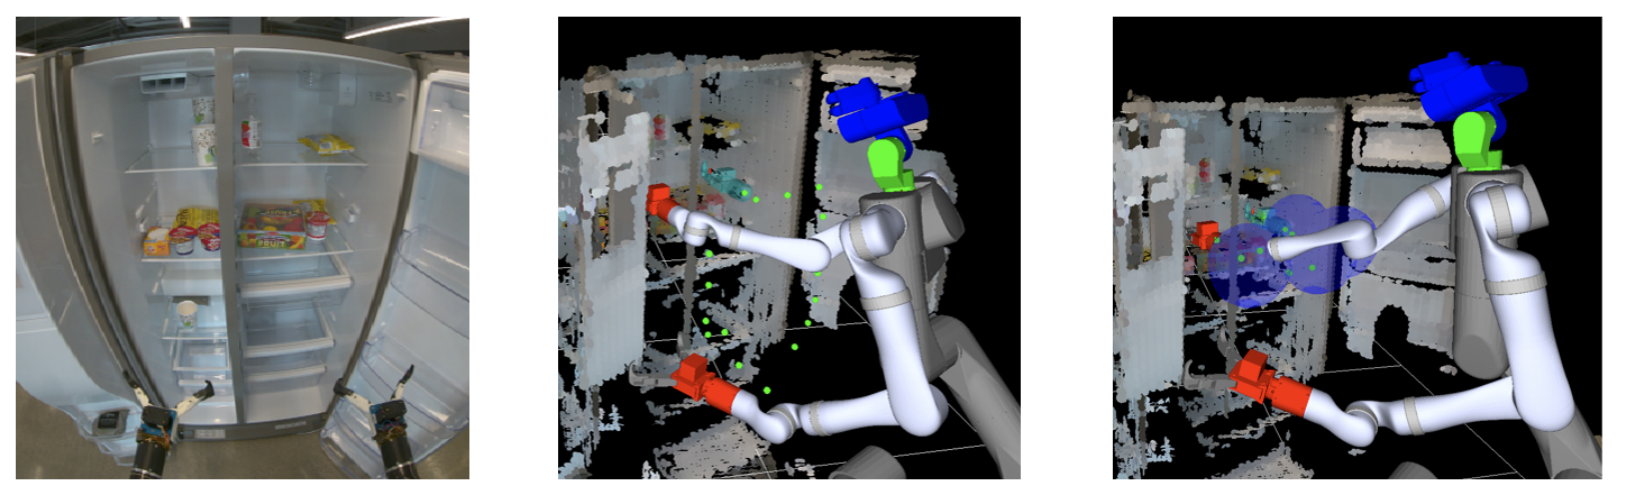
\includegraphics[width=\linewidth]{figures/exampleTask.png}
	\caption[An example of a pick-and-place task]{An example of a robotic manipulation task in a home environment. The green dots signify the planned path for the end effecter to take. \cite{Cheng_Shankar_Burdick_2020}}
	\label{fig:exampleTask}
\end{figure}

\chapter{Background}
This section provides background for each of the individual components of the grasp analyzer.

\section{Center of Mass Estimation}
Humans have an inert ability to estimate the center of mass of common objects through vision alone. This ability enables us to manipulate objects stably as we will minimize the torque generated by a grasp. Conversely, center of mass estimation has also been an important part in the classical (non-learning) approach to grasping \cite{Kanoulas_Lee_Caldwell_Tsagarakis_2018}, \cite{Yong_Yu_Fukuda_Tsujio_1999}. \cite{Yong_Yu_Fukuda_Tsujio_1999} proposed a method that uses the gravity equi-effect plane of an object under external force to determine the center of mass of a polyhedron. However, this method requires the robot to tip the object repeatedly, which may not be feasible in cluttered environments. Moreover, since a lot of common objects are not polyhedrons, the application and accuracy of the method may be limited. \cite{Kanoulas_Lee_Caldwell_Tsagarakis_2018} formulated the process of grasping and finding the center of mass of the object as a reinforcement learning problem. An initial estimate of the CoM (center of mass) is found by finding the centroid of a segmented object's point cloud. Using this CoM, the grasp with the lowest expected torque is executed by the robot and the actual grasp torque is measured by force sensors. This data is then used to re-evaluate the CoM, repeating the procedure until a satisfactory low-torque grasp has been found. This method could lead to irrecoverable failures as a grasp must be executed to calibrate the center of mass found. More importantly, the centroid of a point cloud is not a reliable estimator for center of mass as the full point cloud of an object is usually not attainable in open-world environments. The centroid of partial point cloud may be misleading, causing slippage during grasp.

\section{Grasp Pose Proposer}
Due to the limited contact points provided by a parallel gripper, finding a suitable grasp pose becomes a challenging problem. In recent years, machine learning has become popular approach for grasp proposers \cite{ten_Pas_Gualtieri_Saenko_Platt_2017}, \cite{Mousavian_Eppner_Fox_2019}, \cite{Sundermeyer_Mousavian_Triebel_Fox_2021}. These learning-based methods are able to generate a set of 6-DoF grasp poses for parallel grippers from raw point cloud data. \cite{ten_Pas_Gualtieri_Saenko_Platt_2017} proposed a CNN that is trained using artificial data. The data consists of sampled grasp poses that are labeled as good and bad grasp poses. \cite{Mousavian_Eppner_Fox_2019} proposed a two-part framework where a VAE is trained to sample poses with a point cloud input and an evaluation module is trained to detect and refine the proposed grasps. Contact-GraspNet\cite{Sundermeyer_Mousavian_Triebel_Fox_2021} simplified the representation of grasp poses from 6-DoF to 4-DoF to improve model training. It also used the ACRONYM \cite{Eppner_Mousavian_Fox_2021} dataset, a large simulation-based dataset with a vast amount of different object types. Contact-GraspNet was able to achieve state-of-the-art performance on many benchmarks while being lightweight. It consisted of only one network with a Pointnet++ \cite{Qi2017PointNetDH} encoder backbone and returned directly usable grasp poses. However, since ACRONYM's grasp poses are classified under a zero-gravity environment, the grasp poses generated by Contact-GraspNet do not consider instabilities such as rotation and slippage when the objects' pose change relative to gravity. This leads to the model proposing grasp poses that can be maintained but are unstable. This is shown in \ref{fig:exampleGrasps}.

\begin{figure}
	\centering
	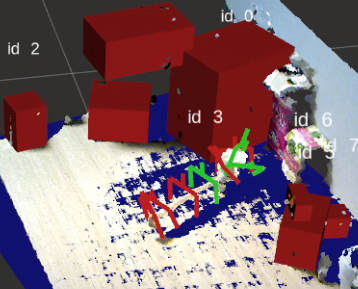
\includegraphics[width=250pt]{figures/grasps.png}
	\caption[Sample grasps from Contact-GraspNet]{Some grasp poses generated by Contact-GraspNet. The red grasp poses are not stable if the object is being lifted, while the green ones are stable lifting grasp poses. The poses are classified by the grasp analyzer proposed.}
	\label{fig:exampleGrasps}
\end{figure}

\section{Grasp Stability Analysis}
The notion of stability has not agreed-upon definition \cite{DBLP:journals/corr/abs-2103-06252}. In certain contexts, stability may refer to the existence of an equilibrium in which the contact point of the object and the gripper obey certain friction laws. With hand-like grippers that provide a high number of contact points, there exists a state of stability where the normal forces of contact completely limit the movement of the object. This is referred to as ``form closure`` \cite{Dizioğlu_Lakshiminarayana_1984} and is a very strong stability condition. An object under form closure is completely kinematically constrained by the contacts of the gripper. Thus unless the motors on the gripper fail, no force in any direction would destabilize the object. However, such analysis would require prior knowledge of the object's shape, which is often unobtainable in open-world settings.

Moreover, in the context of parallel grippers with two pins, it is nearly impossible to achieve form closure. Therefore, it is important for parallel grippers to consider the destabilizing forces and how they affect the grasp under different poses. In an isolated environment where the robot is the only actor,gravity is the only destabilizing force. Thus, given the center of mass of the object and the mass of the object, one can perform simple force and torque analysis to determine the stability of a grasp.


\chapter{Methodology}
The grasp analyzer consists of a grasp proposer, a center of gravity (CoM) estimator, and a grasp classifier \ref{fig:overallPipeline}. The first two components are learning-based; the grasp classifier is a physics-based torque analyzer. For the grasp proposer, a pre-trained version of Contact-GraspNet \cite{Sundermeyer_Mousavian_Triebel_Fox_2021} is used. Contact-GraspNet is chosen for its simplicity as well as its state-of-the-art performance in tabletop scenarios. The CoM estimator and the grasp classifier will be discussed in more details in the following sections.

\begin{figure}
	\centering
	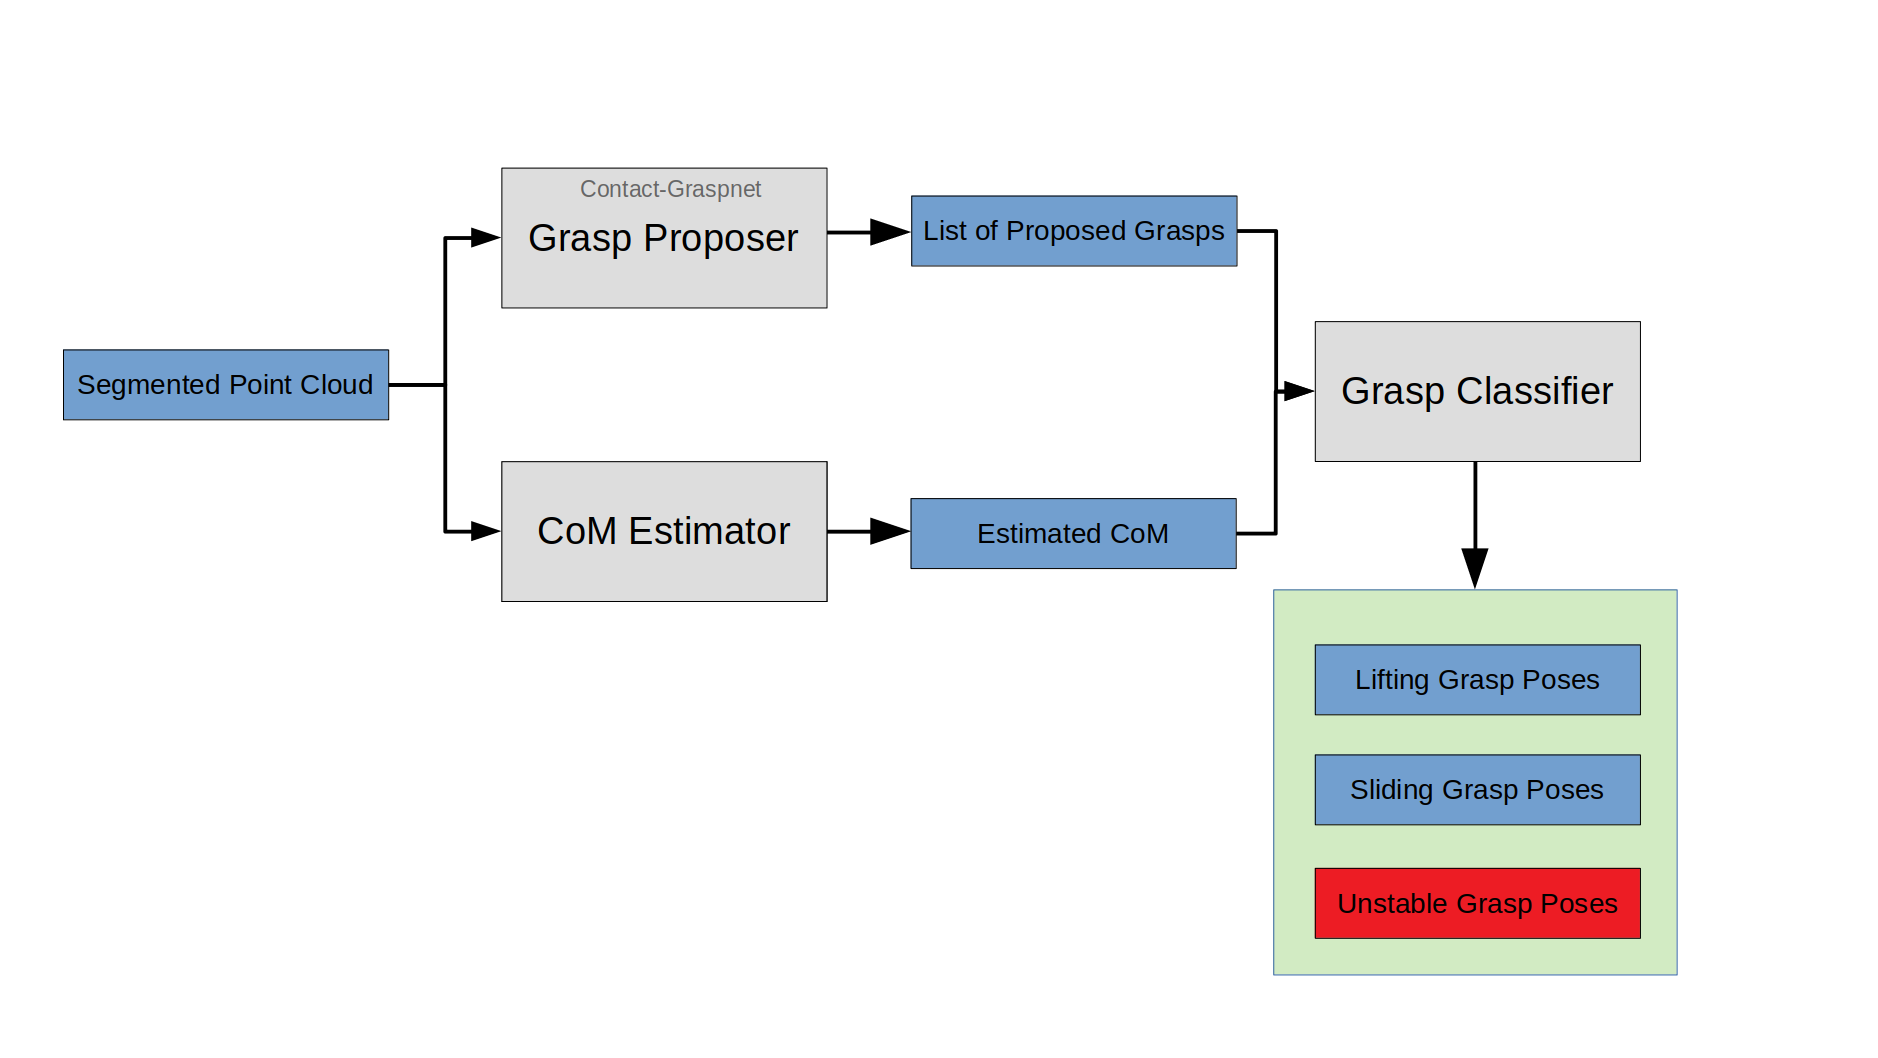
\includegraphics[width=\linewidth]{figures/overallPipeline.png}
	\caption[Overall Pipeline of the proposed grasp analyzer]{The overall pipeline of the grasp analyzer is shown here. The grasp proposer and the CoM estimator take segmented point cloud are input and output a list of proposed grasps and an estimated CoM. The two are then analyzed the grasp classifier to determine which grasps are stable lifting grasps, stable sliding grasps or neither. Note that a grasp can be both a stable lifting grasp and a stable sliding grasp.}
	\label{fig:overallPipeline}
\end{figure}

\section{Center of Mass Estimator}
\subsection{Architecture}
The architecture of the center of mass estimator is shown in \ref{fig:architecture}. Similar to Contact-GraspNet, the first part of the architecture utilizes a Pointnet++ feature extractor to create per-point features from segmented point cloud. This feature is then passed into three fully connected layers. Note that the fully connected layers do not perform reduction to directly generate a CoM estimate. Instead, they produce a ``dense`` (per point) estimate of the CoM as proposed by \cite{wan2017dense}. This has been shown in the pose estimation community to drastically improve the stability and accuracy of estimation from point clouds. In \cite{wan2017dense}, mean shift with consensus is used to aggregate the per-point estimations. However, in the setting of center of mass estimation, using mean shift or RANSAC did not show any improvement in accuracy. Therefore, a simple averaging is used to aggregate the dense estimates to form the final center of mass estimation.

\begin{figure}
	\centering
	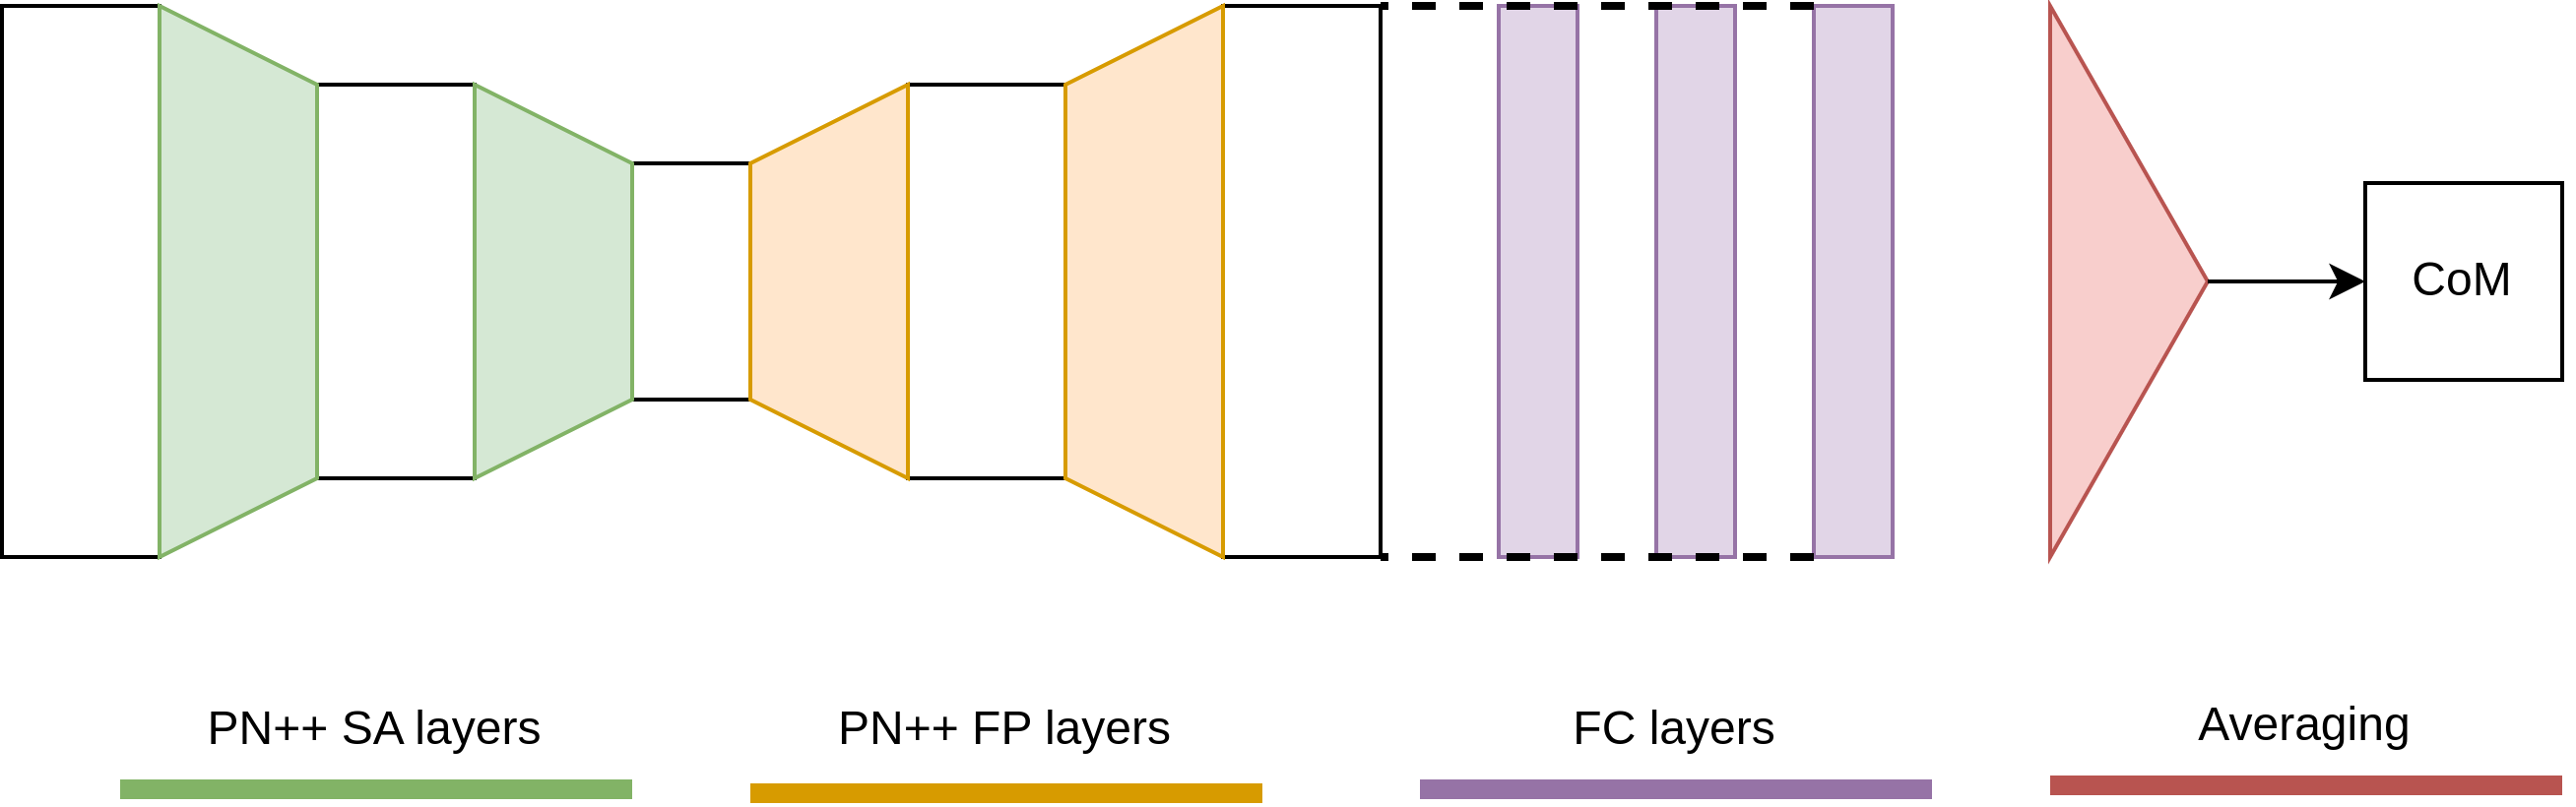
\includegraphics[width=\linewidth]{figures/Architecture.png}
	\caption[Architecture of the center of mass estimator]{The architecture of the center of mass estimator is shown here. The first part of the network is a point cloud feature extractor with three Pointnet++ Set Abstraction layers and three Pointnet++ Feature Propagation layers. The per-point features are then fed into three fully connected layers. As the layers do not reduce in dimensions, they can also be viewed as convolution layers. The fully connected layers produce estimates of the object's center of mass for each point in the point cloud.}
	\label{fig:architecture}
\end{figure}

\subsection{Point Cloud Augmentation}
The aforementioned architecture achieves a satisfactory performance in terms of overall accuracy. However, there are some egregious failure cases such as predicting CoMs that are below the table as shown in \ref{fig:failExample}. To remedy these errors, an ``imagined`` table point cloud is added similar to \cite{qin2022dexpoint}. In \cite{qin2022dexpoint}, an imaginary hand point cloud is added to improve the model's cognition of the spatial relationship between the hand and the manipulation target. In the case of CoM estimation, the imaginary table surface point cloud serves a similar purpose. It allows the model to get a better sense of the size of the object even under occlusion. It also allows the model to better assess the the placement of the object on the table. Given that the object must be in a stable placement, additional assumptions about the object's distribution of mass can be made to help with center of mass prediction. With the imaginary table surface point cloud added to augment the segmented partial point cloud of the objects, egregious errors with CoM estimations decreases significantly.

\begin{figure}
	\centering
	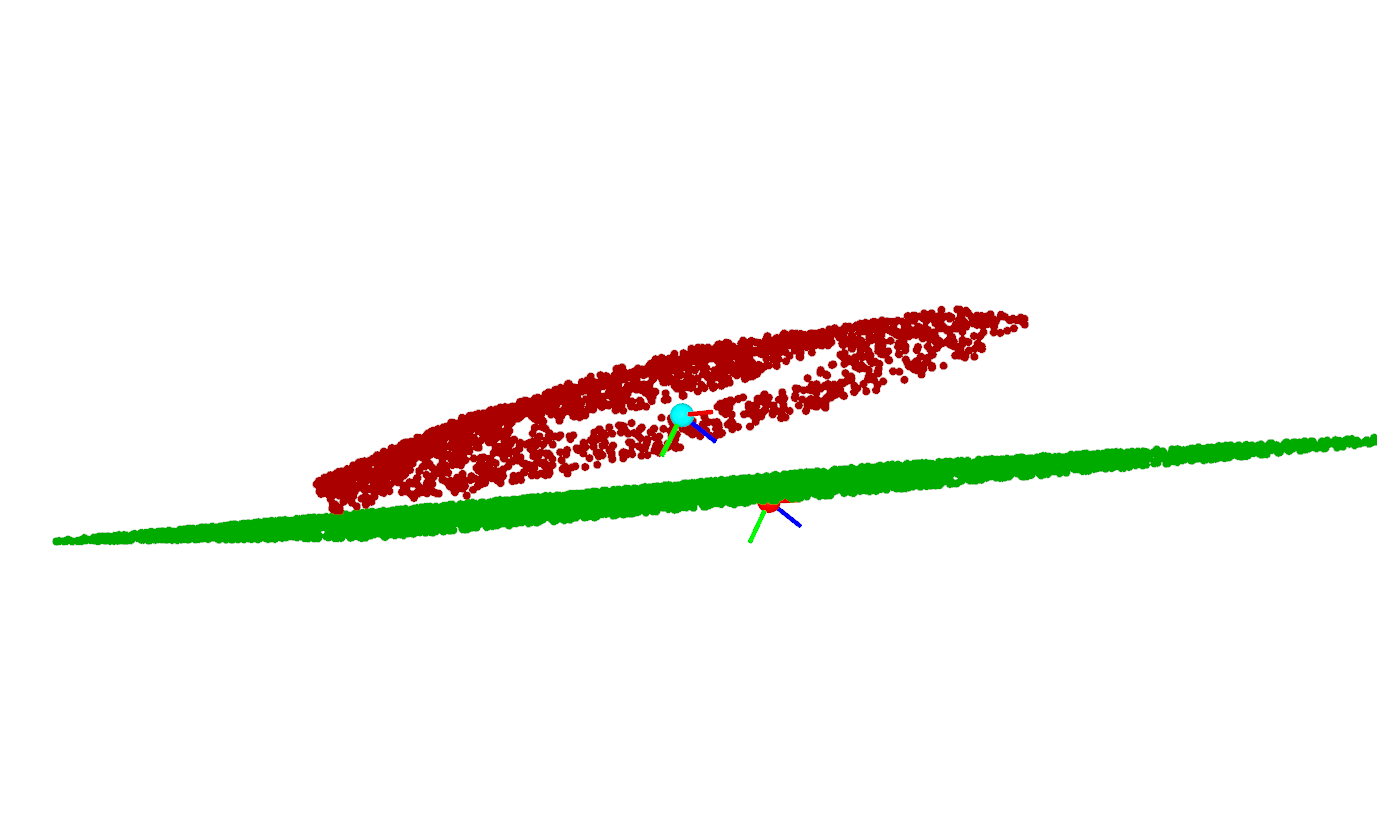
\includegraphics[width=0.6\linewidth]{figures/failExample.png}
	\caption[An example failure with unaugmented point cloud as input]{An example of estimation failure. The ground truth center of mass if shown in blue while the predicted center of mass is shown in red. The object's observed point cloud is shown in red and the table is shown in green. Because only the partial object point cloud is passed to the model, the model is unsure of the exact dimensions of the object and makes a prediction that overestimates the size of the object.}
	\label{fig:failExample}
\end{figure}

\subsection{Data Set and Training}
The model is trained using a data set derived from the ACRONYM database \cite{Eppner_Mousavian_Fox_2021}. ACRONYM contains center of mass information of ShapeNet \cite{chang2015shapenet} objects. ACRONYM's toolkit also contains methods that allows the user to generate tabletop scenes. A total of 1000 scenes are generated by placing a random object in a random stable placement on a table. For each scene, five different camera angles that resemble a robot's view of the tabletop are created randomly. Each camera angle would generate a distinct partial point cloud of the object. Each partial point cloud is augmented with a labeled imagined tabletop point cloud; center of mass and a camera matrix annotations are also included. An example of the five point clouds from a different scenes are shown in \ref{fig:PCExamples}. Of the 5000 samples, 4000 are used to train the model and 1000 are reserved for evaluation.

The model is trained with a learning rate of 0.001 using the ADAM optimizer. The loss function is the average L2 loss of the dense predicted CoM and the ground truth CoM. The final model achieves an average CoM estimation error of $2\mathrm{cm}$ on the evaluation data set. Some example predictions are shown in \ref{fig:PredExamples}.

\begin{figure}
	\centering
	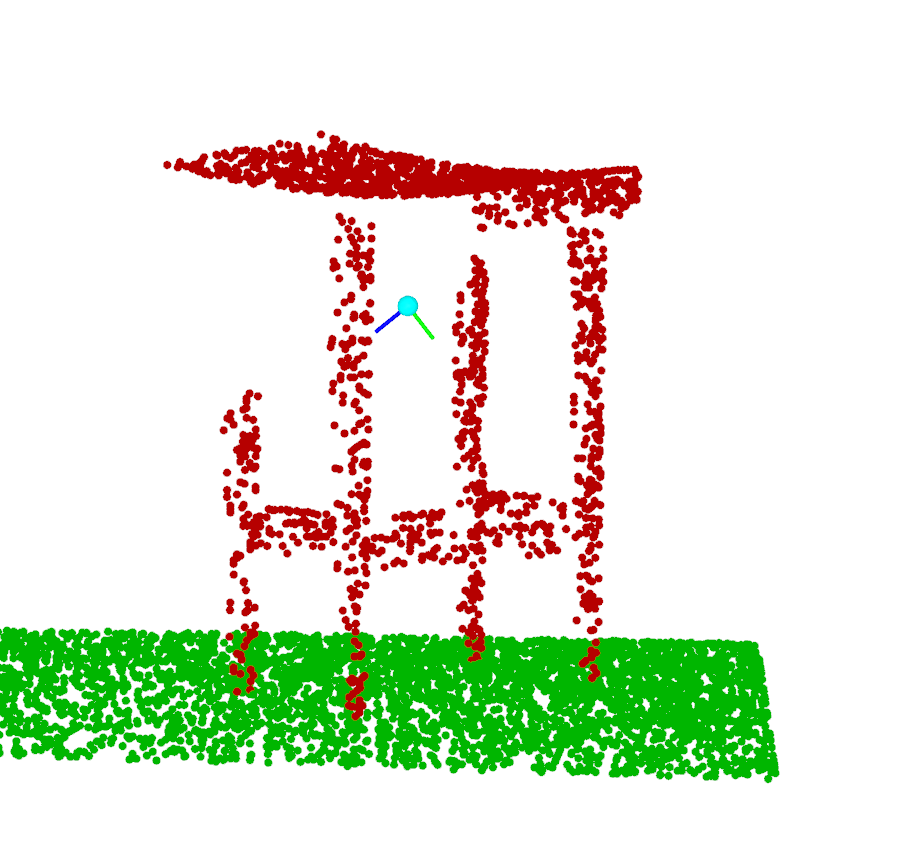
\includegraphics[width=0.19\linewidth]{figures/ex1.png}
	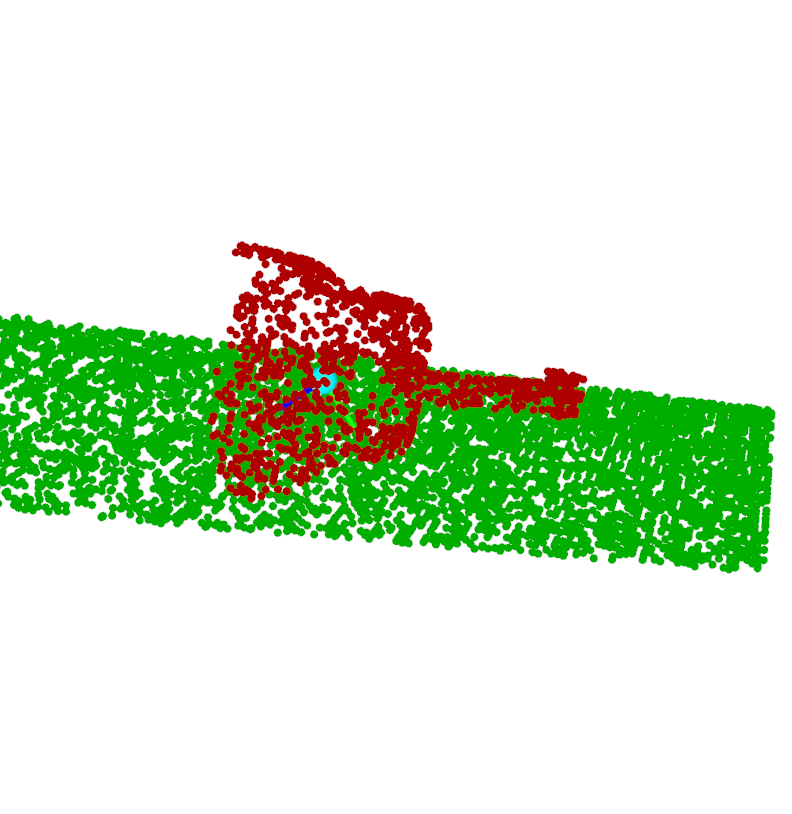
\includegraphics[width=0.19\linewidth]{figures/ex2.png}
	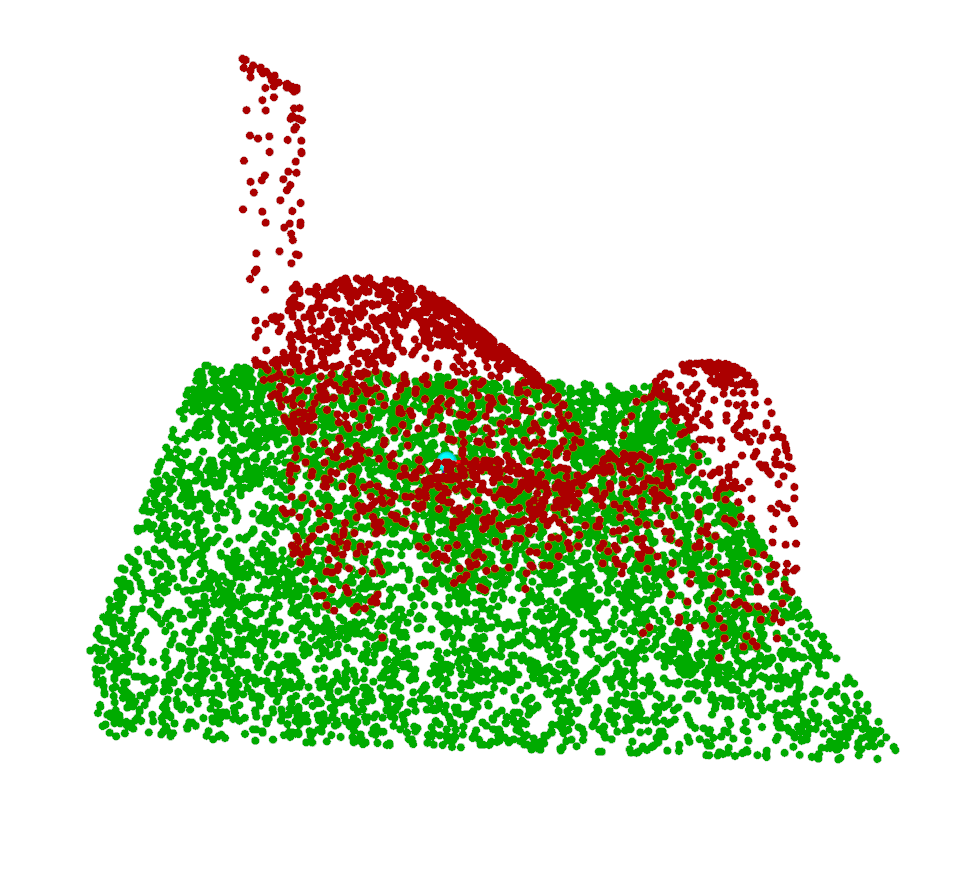
\includegraphics[width=0.19\linewidth]{figures/ex3.png}
	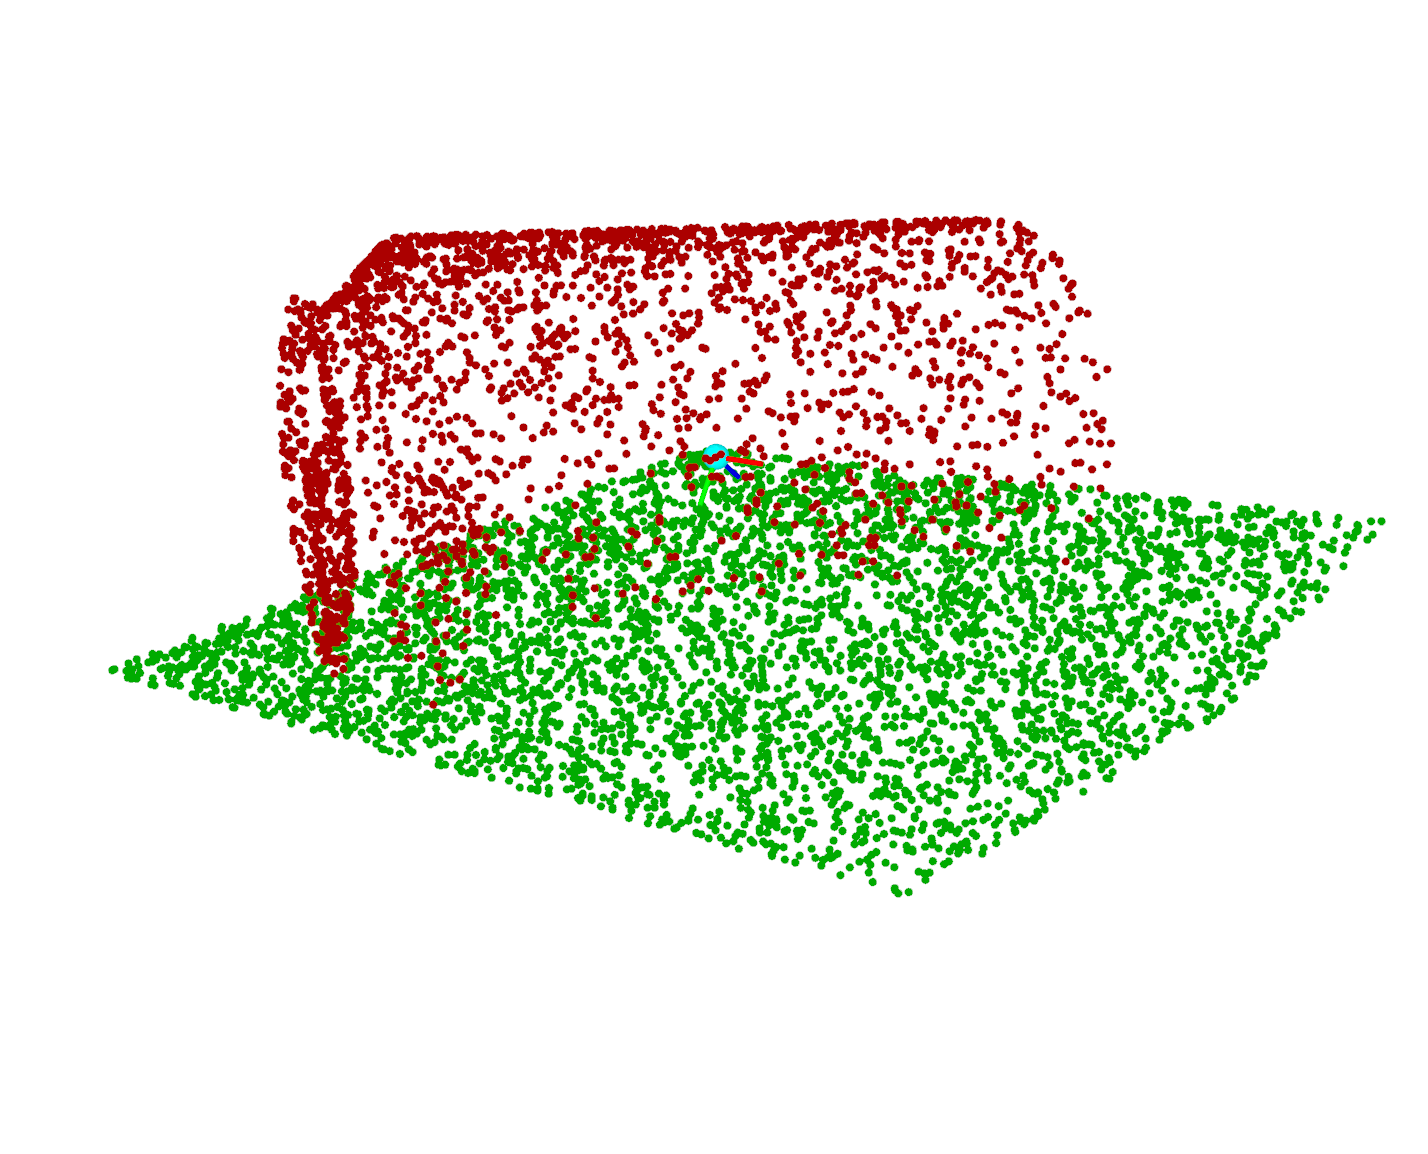
\includegraphics[width=0.19\linewidth]{figures/ex4.png}
	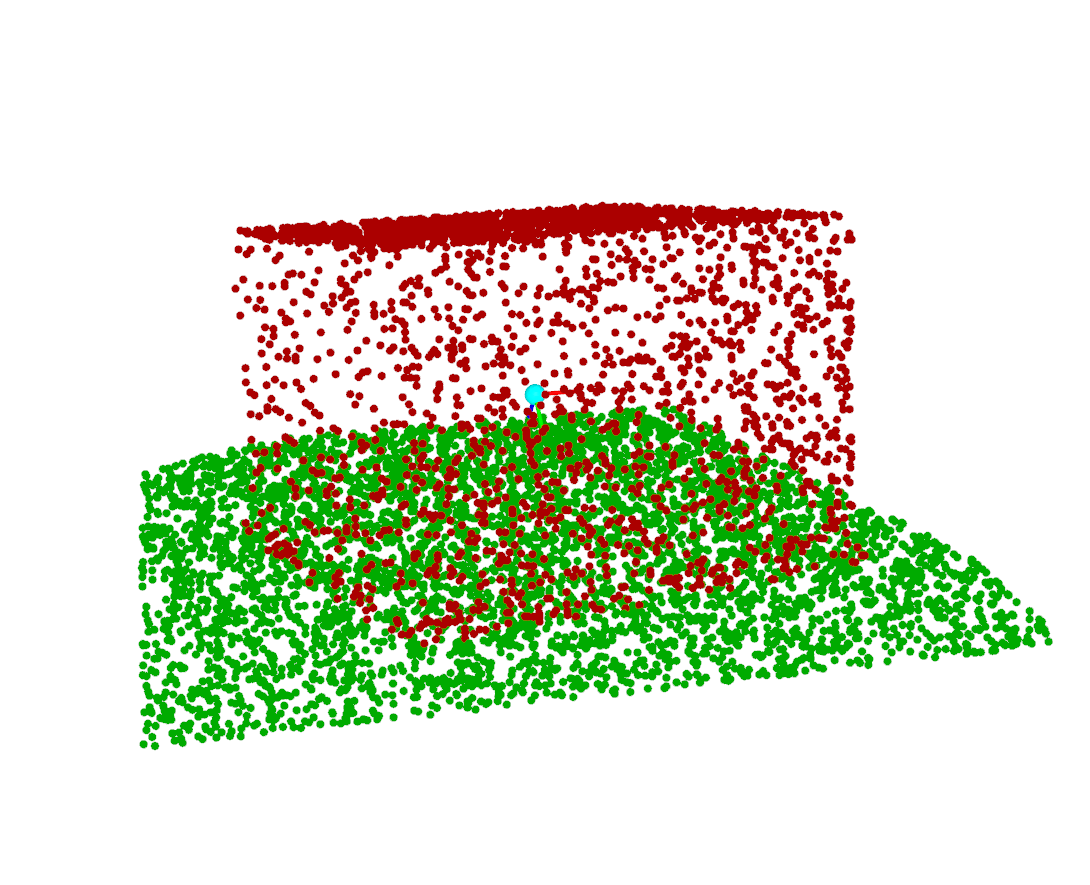
\includegraphics[width=0.19\linewidth]{figures/ex5.png}
	\caption[Examples of different object from different scenes]{Examples of generated data with partial object point cloud in red, augmented table point cloud in green, ground truth center of mass as a blue dot. The axis shown on the ground truth center of mass is aligned with the camera reference frame.}
	\label{fig:PCExamples}
\end{figure}

\begin{figure}
	\centering
	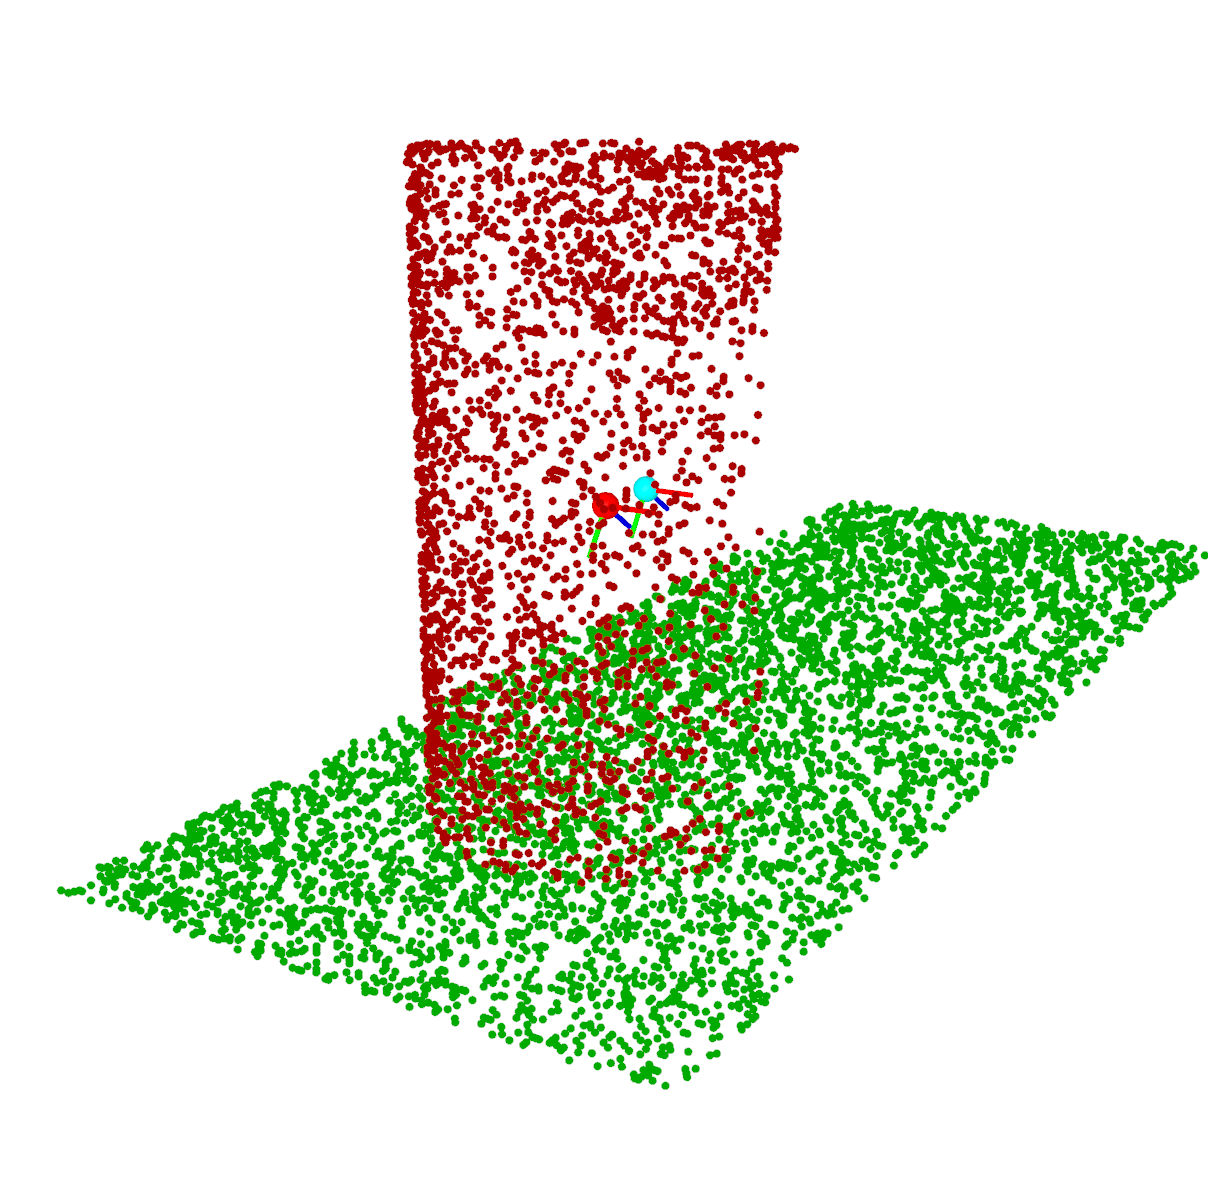
\includegraphics[width=0.19\linewidth]{figures/pred1.png}
	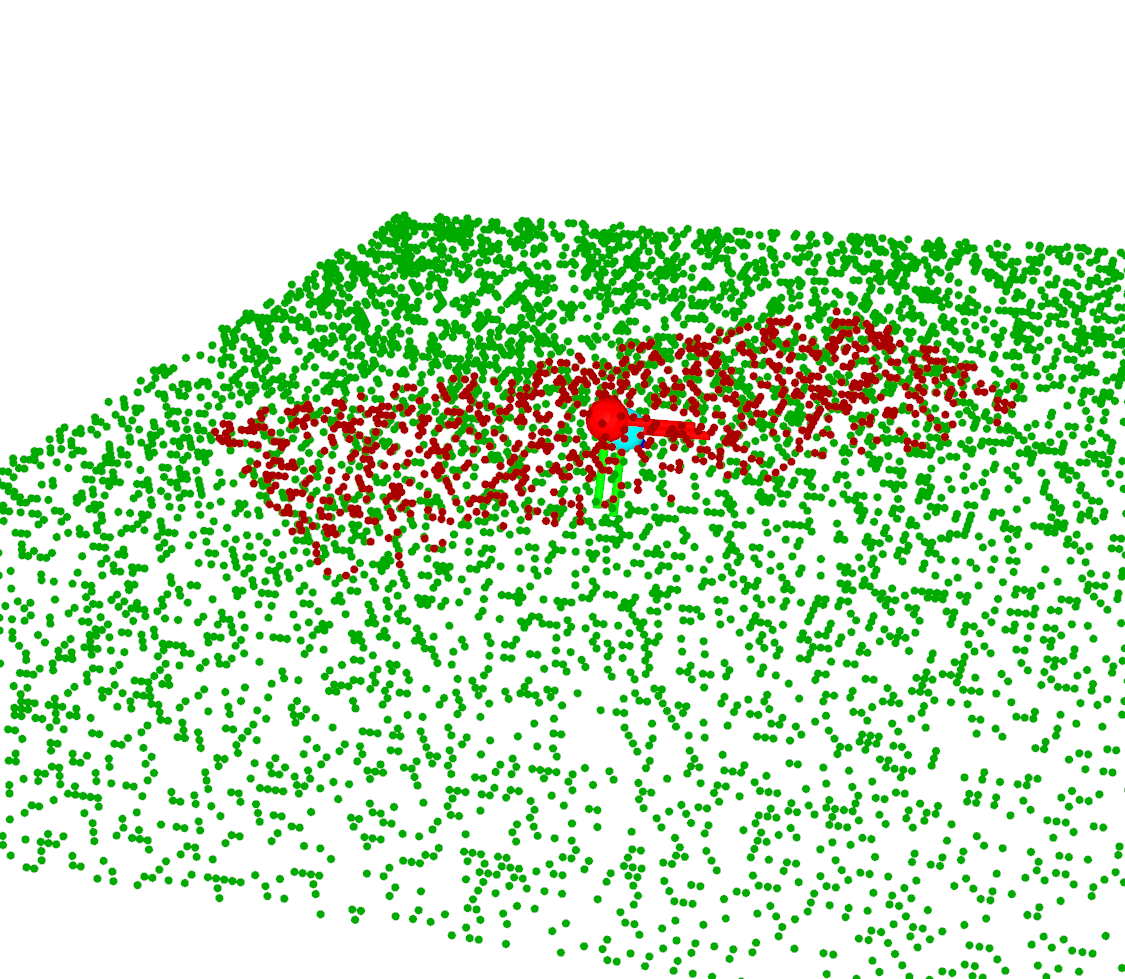
\includegraphics[width=0.19\linewidth]{figures/pred2.png}
	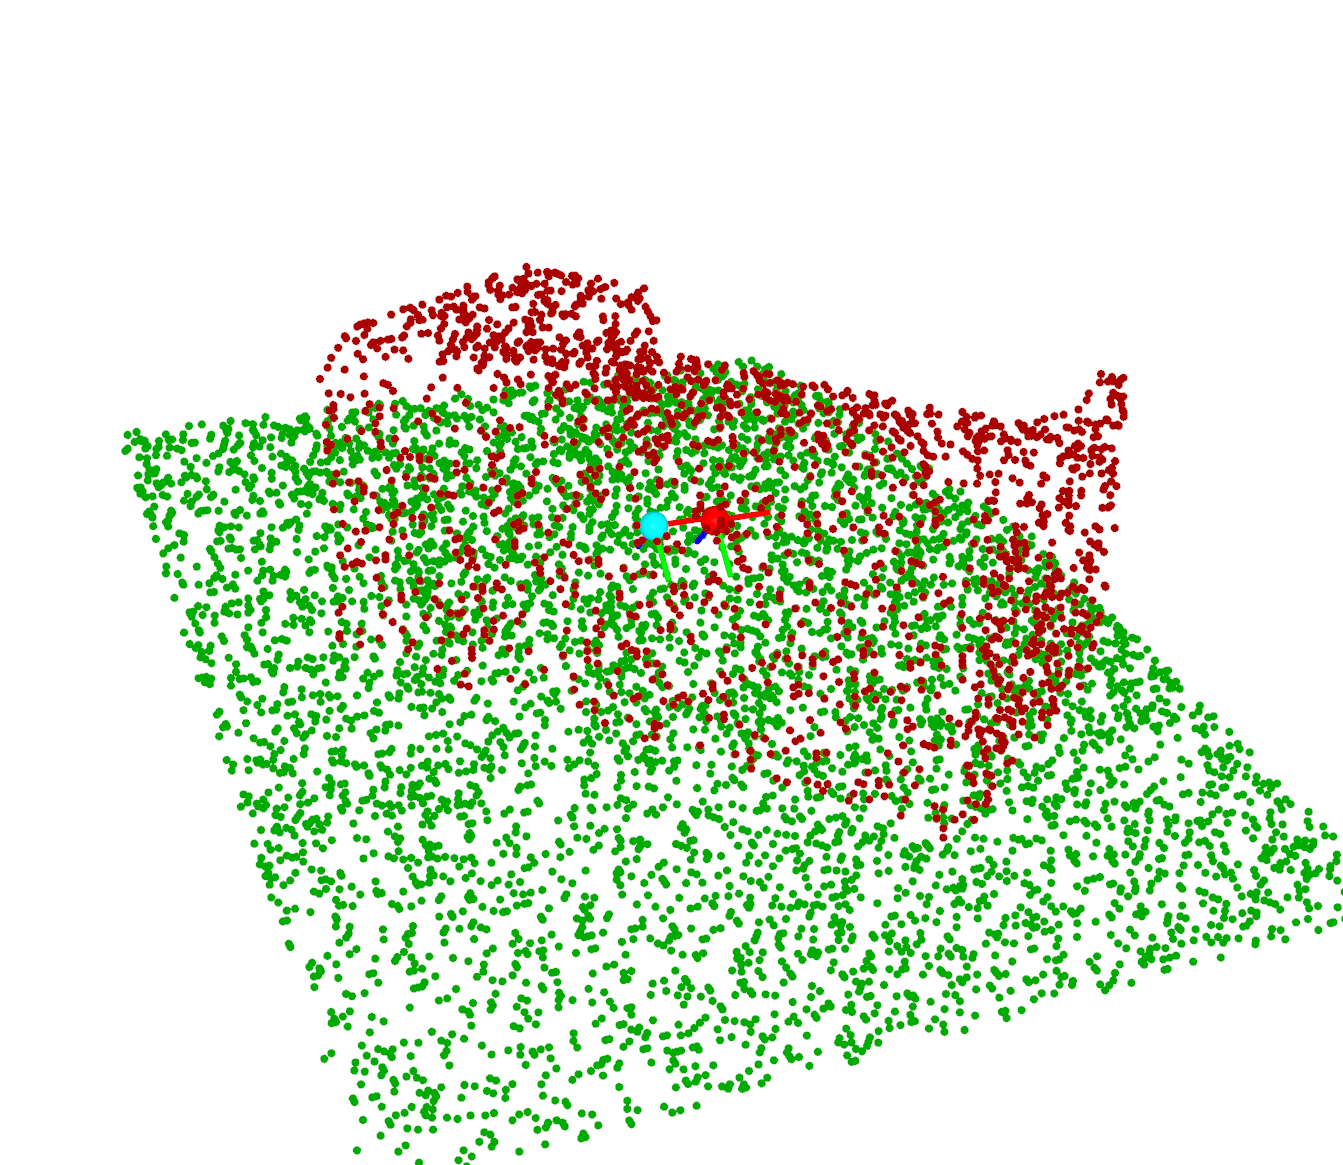
\includegraphics[width=0.19\linewidth]{figures/pred3.png}
	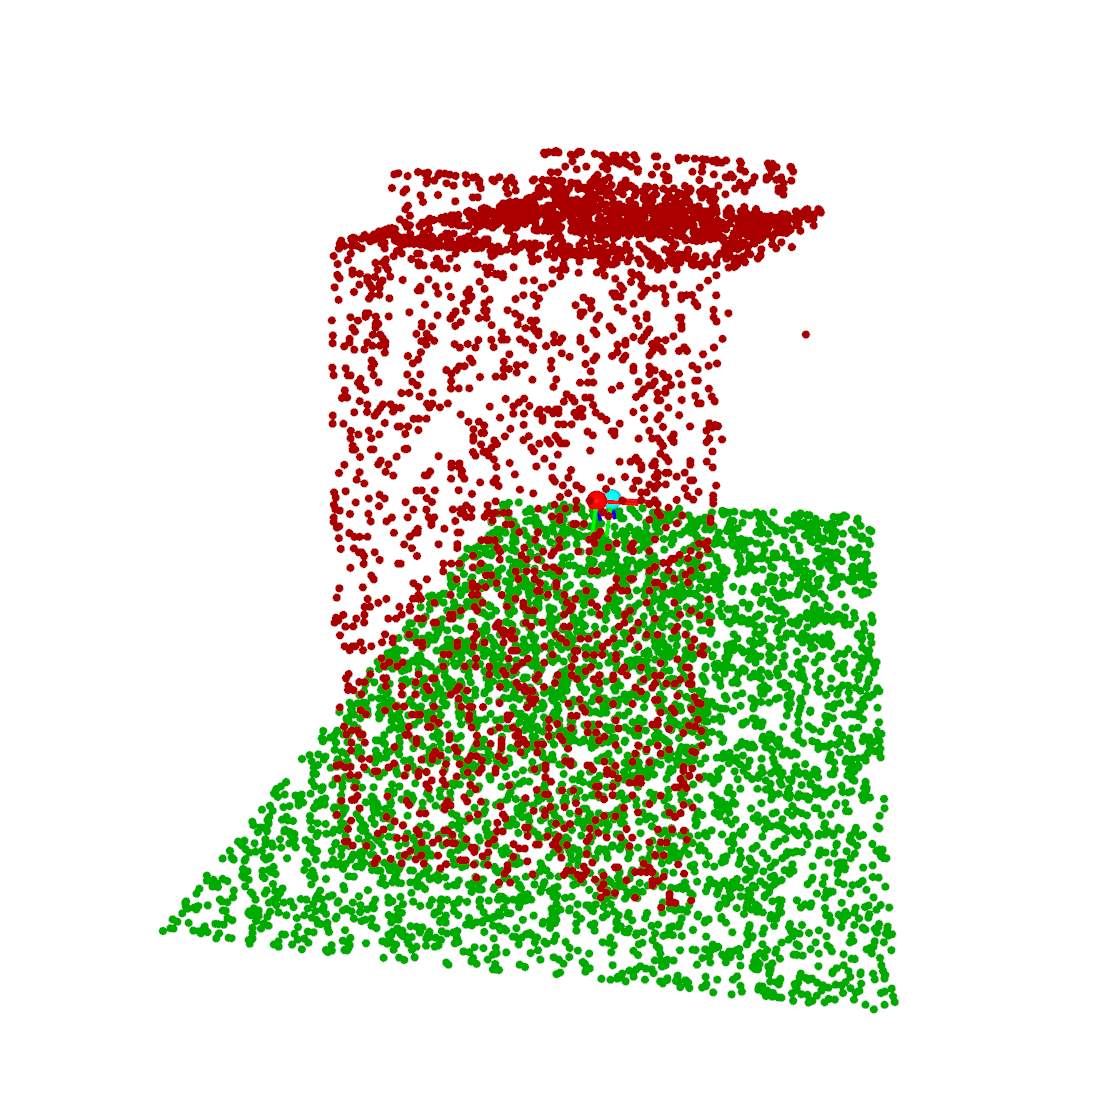
\includegraphics[width=0.19\linewidth]{figures/pred4.png}
	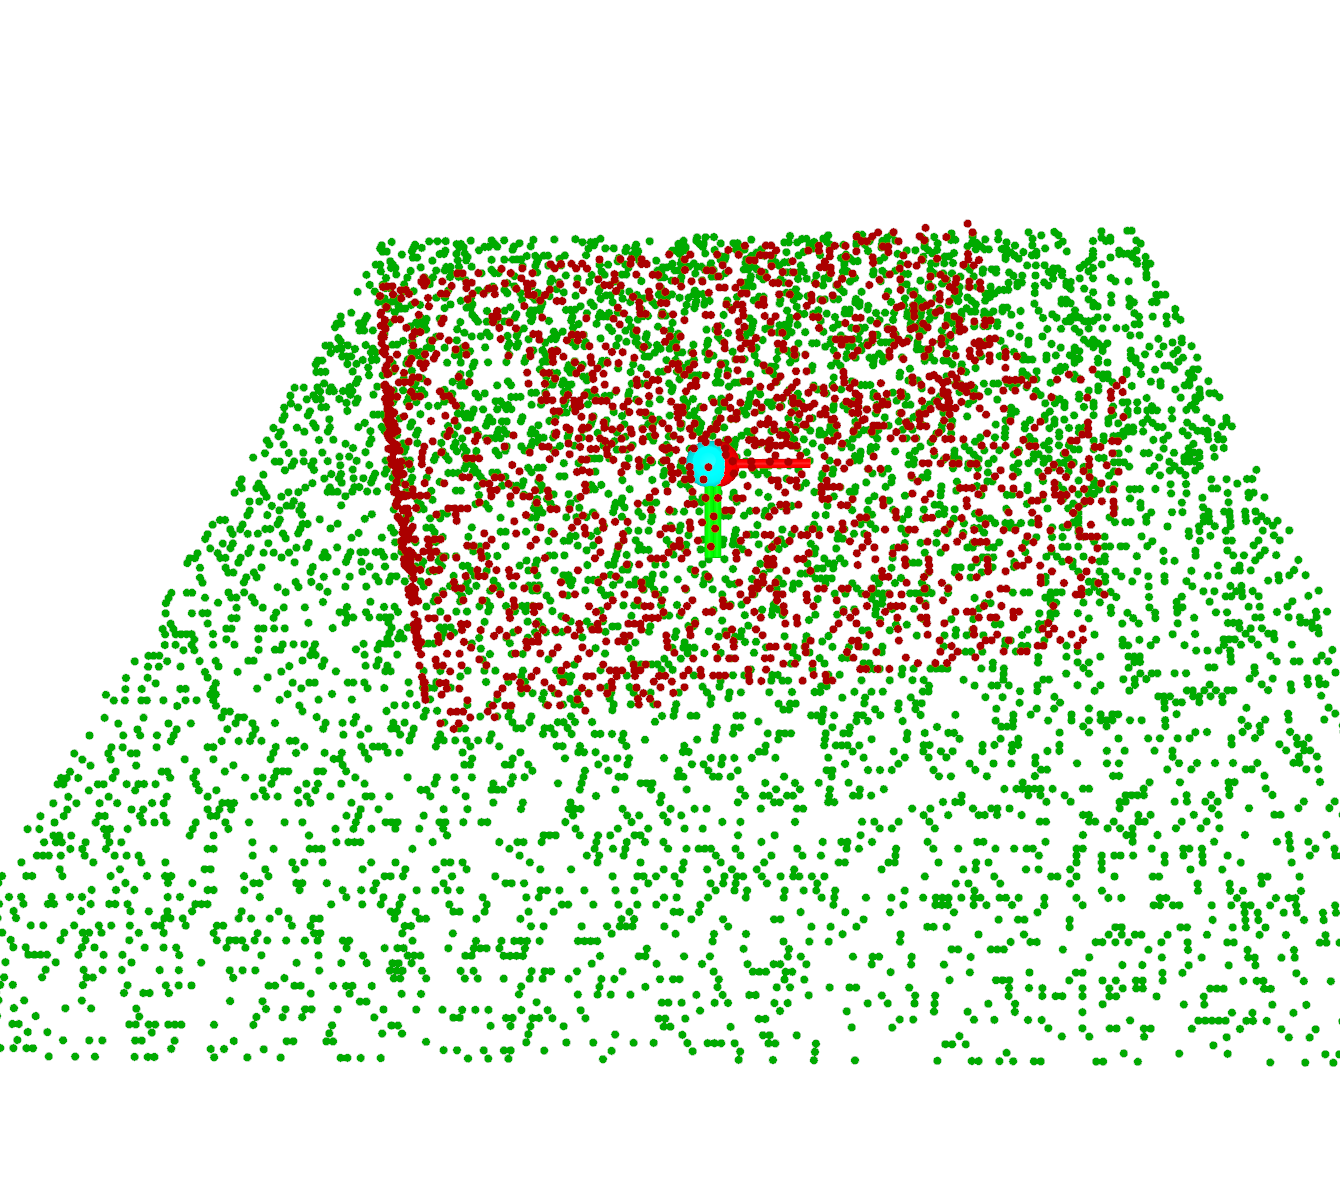
\includegraphics[width=0.19\linewidth]{figures/pred5.png}
	\caption[Examples of predicted center of mass]{Examples of prediction results. The ground true center of mass is shown as a blue dot while the predicted center of mass is shown as a red dot.}
	\label{fig:PredExamples}
\end{figure}


\section{Grasp Classifier}
\subsection{Assumptions}
This work assumes that the parallel gripper has only two pins with powerful motors. This work also assumes that the manipulation task is in isolation, meaning that the robot is the only actor in the task. In such context, the forces acting on the object are gravity and the contact forces exerted by the two pins as well as the resulting friction.

A stable grasp for lifting is defined as when the object is lifted by the grasp, the relative pose between the gripper and the object does not change; vice versa, a stable grasp for sliding is defined as when the object is slid by the grasp, the relative pose between the gripper and the object does not change. 

Under this setting, it is possible to classify grasp destabilization as two types: slippage destabilization and rotational destabilization. Slippage destabilization refers to the scenario when the contact friction between the gripper and the object is not sufficient to support the object's weight. Rotational destabilization refers to the the scenario when the static torque between the gripper and the object is not sufficient to balance out the object's gravitational torque. The two types of destabilization are illustrated for the lifting case in \ref{fig:liftIllustrations} and for sliding case in \ref{fig:slideIllustrations}. 

It is assumed that slippage destabilization does not happen for any of the grasps proposed. This assumption is based on three reasons. First, grasps generated by Contact-GraspNet are usually immune to slippage as the network is trained to prevent such destabilization. Second, the motors on the gripper are usually very powerful. Thus, in practice, the maximum friction and normal forces generated by the gripper usually far exceed the gravitational forces and the friction between the object and the table. Finally, if slippage destabilization is possible, it usually means that the object is too heavy or has a very high friction coefficient for the gripper to handle. If that is the case, grasp analysis become a moot point as the robot simply lacks enough power to manipulate the object.

Given the above assumptions, the focus of the grasp classifier is therefore to analyze the torques in play to prevent rotational destabilization during manipulation.

\begin{figure}
	\centering
	\begin{subfigure}[b]{0.4\linewidth}
		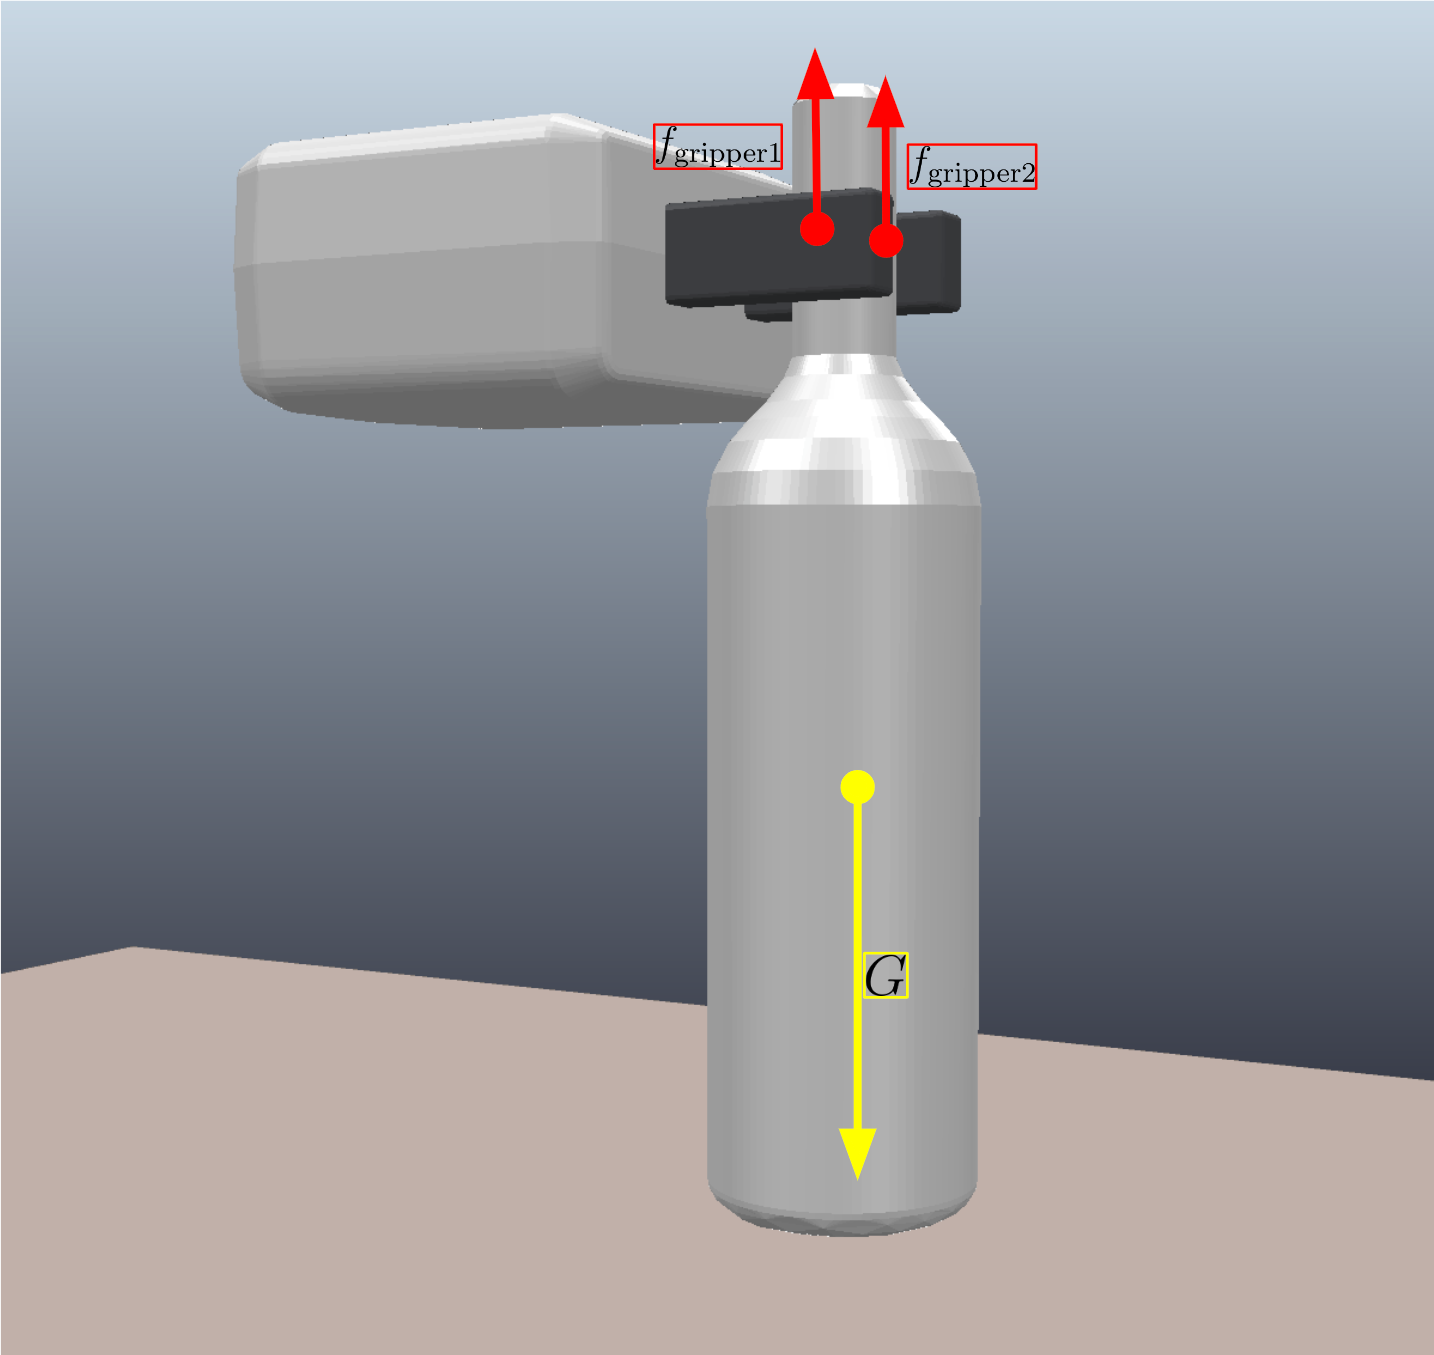
\includegraphics[width=\linewidth]{figures/slippage.png}
		\caption{Slippage}\label{liftfiga}
	\end{subfigure}%
	\hfill
	\begin{subfigure}[b]{0.4165\linewidth}
		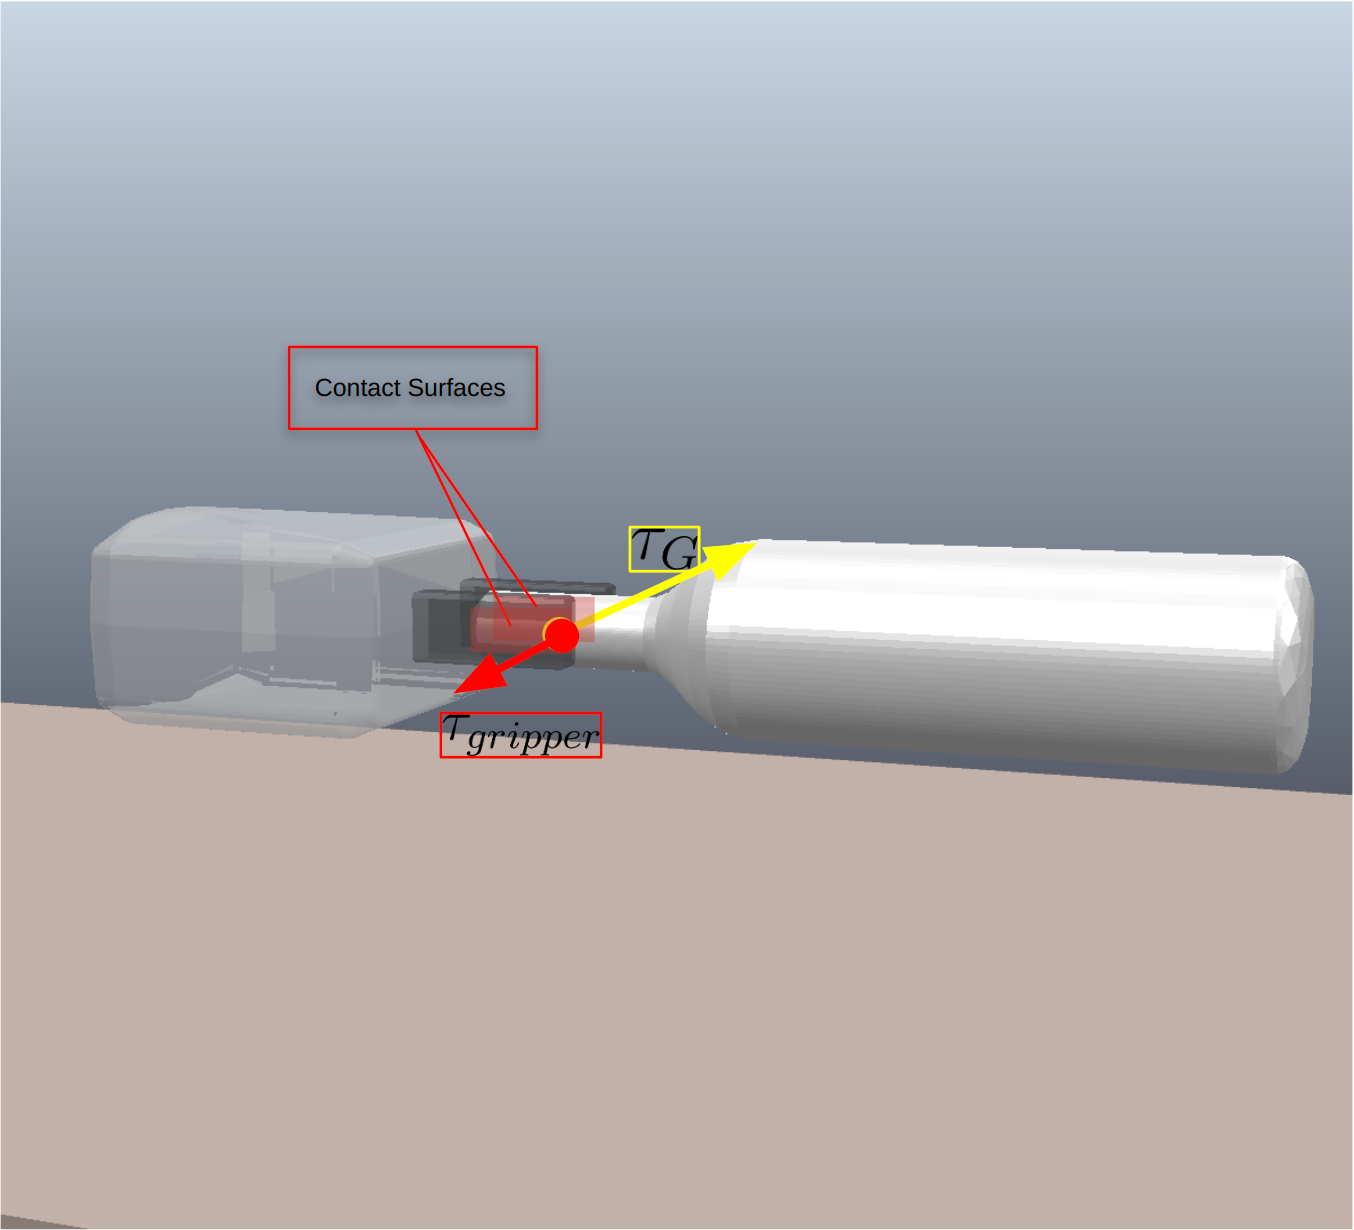
\includegraphics[width=\linewidth]{figures/rotational.png}
		\caption{Rotational}\label{liftfigb}
	\end{subfigure}%
	\caption[Slippage and rotational destablization illustrations for lifting grasps.]{(a) shows the forces in play for a lifting grasp concerning slippage destabilization. $f_{\mathrm{gripper1}}$ and $f_{\mathrm{gripper2}}$ are the static friction exerted by each of the two gripper pins; $G$ is the gravitational force experience by the object. (b) shows the torques in play for a lifting grasp concerning rotational slippage. By choosing the center of grasp as pivot, $\tau_{gripper}$ is the static torque created by the contact surface between the gripper and the object; $\tau_G$ is the gravitational torque experienced by the object.}
	\label{fig:liftIllustrations}
\end{figure}

\begin{figure}
	\centering
	\begin{subfigure}[b]{0.45\linewidth}
		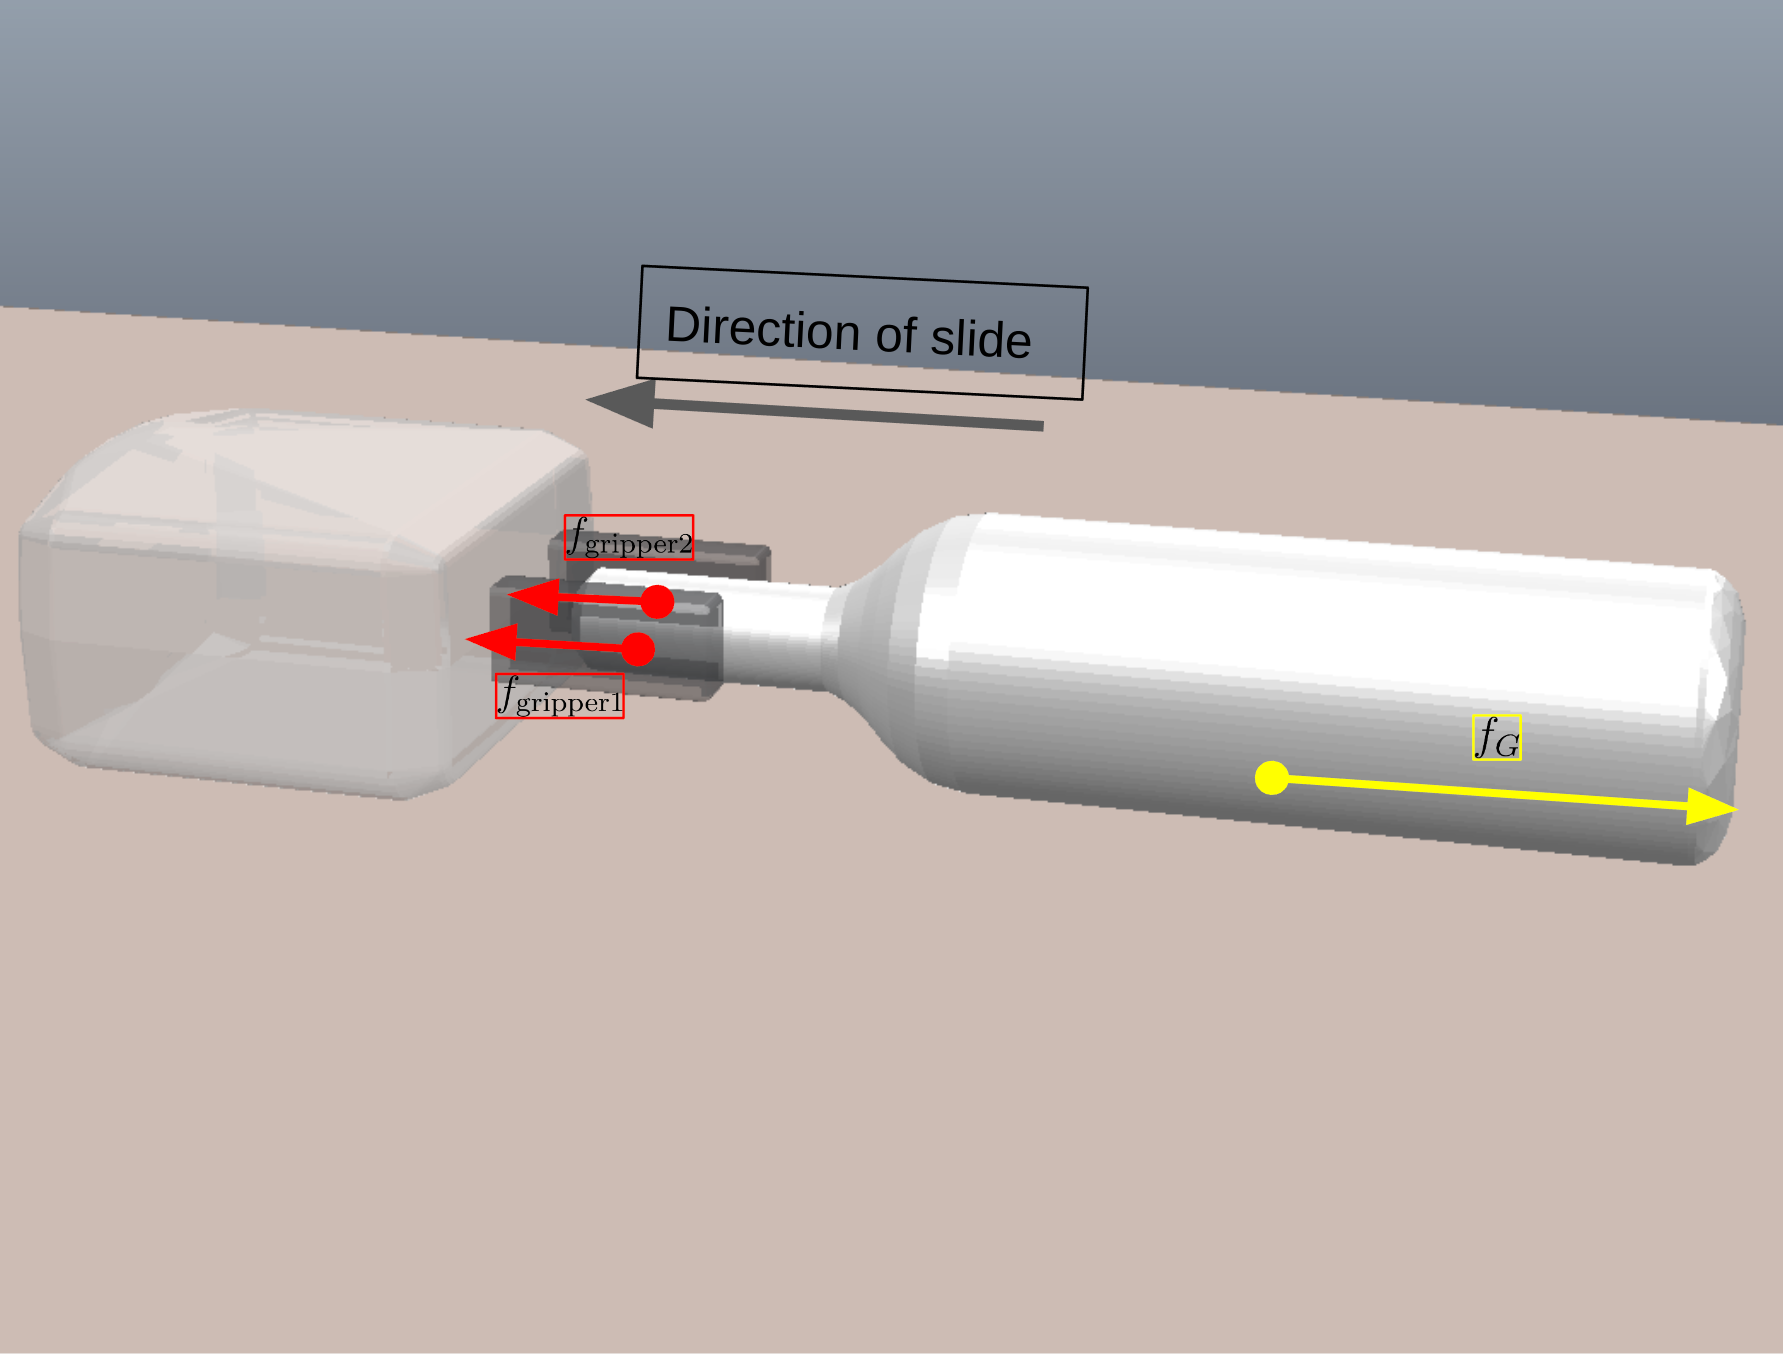
\includegraphics[width=\linewidth]{figures/slideSlippage.png}
		\caption{Slippage}\label{slidefiga}
	\end{subfigure}%
	\hfill
	\begin{subfigure}[b]{0.407\linewidth}
		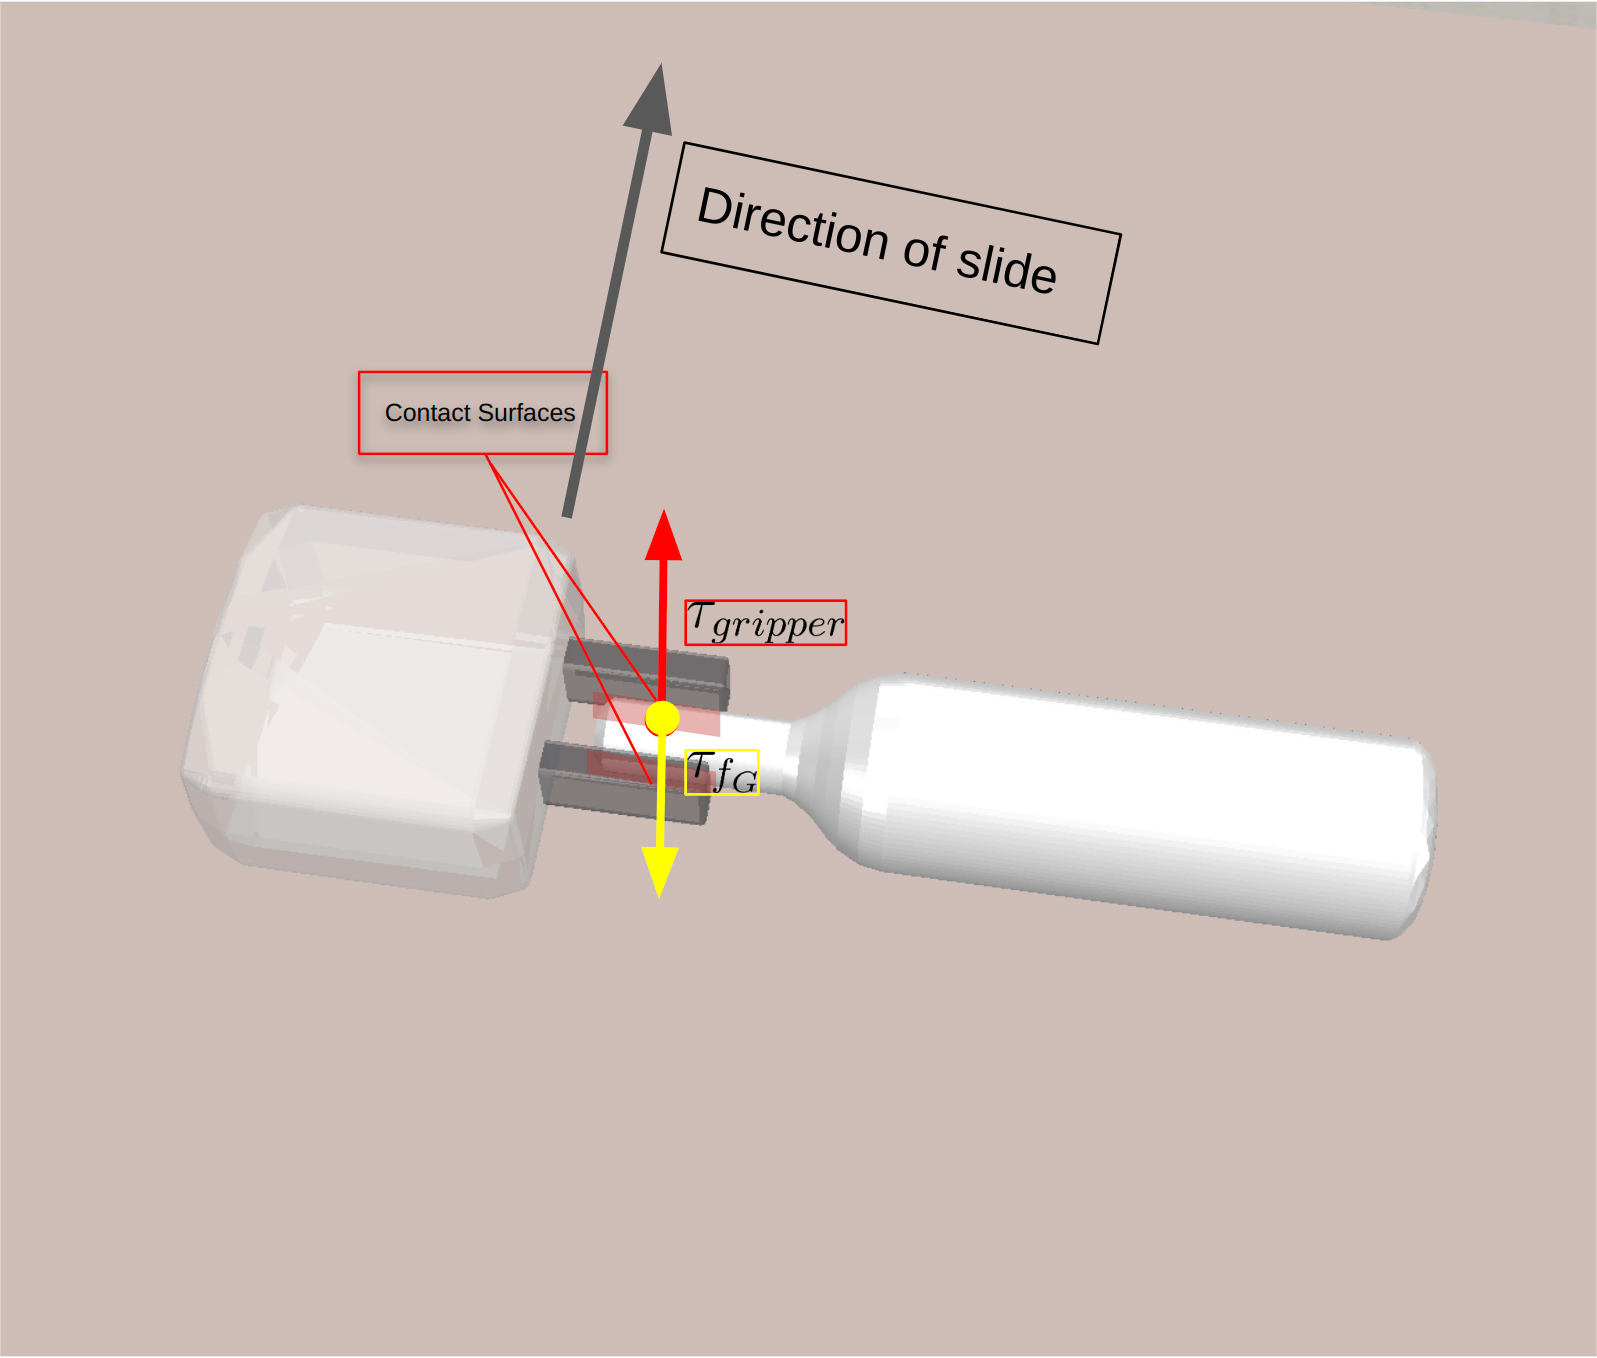
\includegraphics[width=\linewidth]{figures/slideRotation.png}
		\caption{Rotational}\label{slidefigb}
	\end{subfigure}%
	\caption[Slippage and rotational destablization illustrations for sliding grasps.]{(a) shows the forces in play for a sliding grasp concerning slippage destabilization. The object is being slid to the left. $f_{\textrm{gripper1}}$ and $f_{\textrm{gripper2}}$ are the static friction exerted by each of the two gripper pins; $f_G$ is the friction caused by gravitational force experience by the object. (b) shows the torques in play for a sliding grasp concerning rotational slippage. The object is being slid upwards. By choosing the center of grasp as pivot, $\tau_{gripper}$ is the static torque created by the contact surface between the gripper and the object; $\tau_{f_G}$ is the torque experienced by the object due to the friction between it and the table.}
	\label{fig:slideIllustrations}
\end{figure}



\subsection{Model and Notions}
An accurate model for torque analysis would be intractable. For instance, pivot point selection in non-equilibrium systems become complicated. Therefore, most approaches such as \cite{Kanoulas_Lee_Caldwell_Tsagarakis_2018} simply consider grasps with smaller distances to the center of mass as stable grasps. However, such models neglect two-pinned parallel grippers generate vastly different static torques in different axis.  For instance, the maximum static torque generated by the gripper in \ref{liftfigb} would be much smaller than the in \ref{slidefigb}, and this would lead to a rotation in \ref{liftfigb} while the grasp in \ref{slidefigb} would remain stable.

To model this property while keeping calculations tractable, maximum static torque is defined as three separate values on each of the three axis for a Fetch \cite{Wise2016FetchF} gripper \ref{fig:torqueFrame}. The pivot point is selected as the center of grasp, denoted as the origin in \ref{fig:torqueFrame}. As slippage destabilization is unlikely to happen, this pivot point is a good approximation to the actual pivot point of the object when motion is relatively low-velocity. The maximum static torque on each axis is denoted as $\tau_{\mathrm{max}}^x$, $\tau_{\mathrm{max}}^y$ and $\tau_{\mathrm{max}}^z$ respectively. The torque generated by either the gravitational force or friction between object and table is denoted as $\tau_{\mathrm{rotation}}$. This torque can be found with a simple cross product:
\[
\begin{aligned}
\tau_{\mathrm{rotation}} &= L_{\mathrm{rotation}} \times F_{\mathrm{rotation}}\\
						&= ( P_{\mathrm{rotation}} - P_{\mathrm{GraspCenter}} ) \times F_{\mathrm{rotation}}
\end{aligned}
\]

Where the $L_{\mathrm{rotation}}$ is the lever arm and $F_{\mathrm{rotation}}$ is the rotational force (gravitation force or friction). $L_{\mathrm{rotation}}$ is found by the displacement between the object's grasp center and the rotational force's point of exertion.

The rotational torque is then decomposed into the gripper's reference frame via a vector-matrix multiplication

\[
 \begin{bmatrix}
\tau_{\mathrm{rotation}}^x \\
\tau_{\mathrm{rotation}}^y \\
\tau_{\mathrm{rotation}}^z
\end{bmatrix}  
= 
 \begin{bmatrix}
\textbf{x} \\
\textbf{y} \\
\textbf{z}
\end{bmatrix} 
\cdot
\tau_{\mathrm{rotation}}
\]

where $\begin{bmatrix}
\textbf{x} \\
\textbf{y} \\
\textbf{z}
\end{bmatrix} $ represents the orthogonal normal matrix of the gripper's reference frame. The rotation torque in each axis is then compared to the maximum static torque in each axis to determine the grasp pose's stability. If none of the rotational torques in any direction exceeds the maximum static torque, the pose is deemed stable. Otherwise, it is deemed unstable. An example is shown in \ref{fig:classificationExample}.

\subsection{Additional Details}
For lifting grasp poses, since gravitational force only has one direction, torque analysis only needs to be performed once. For sliding grasp poses, since the frictional force's direction depends on the direction the object is being slid, a single torque analysis is not sufficient. For each sliding pose, a number of directions are sampled uniformly from $2\pi$ and each direction is analyzed. A sliding pose is stable only if all directions have stable torques. The sampling density is a parameter that can be tuned. For sliding poses analysis, the exact point on which of the friction is exerted is also unknown. Ideally, it can be found by integrating over the mass distribution and the friction coefficient of the object. In practice, this point can be estimated as the projection of the center of mass of the object onto the table. This is true if the object's friction coefficient is even across the contact surface.

In practice, the mass of the object, the friction coefficient and the maximum static torques of the gripper are unknown. Therefore, it is impossible to give exact classification. Instead, in practice, the grasp poses are first clustered to reduce their number. Then, each pose is ranked based on their torque analysis results. The top ranked poses are classified as stable poses. The clustering process allows for a diverse set of grasps to be recommended. Both clustering and ranking parameters can be tuned.


\begin{figure}
	\centering
	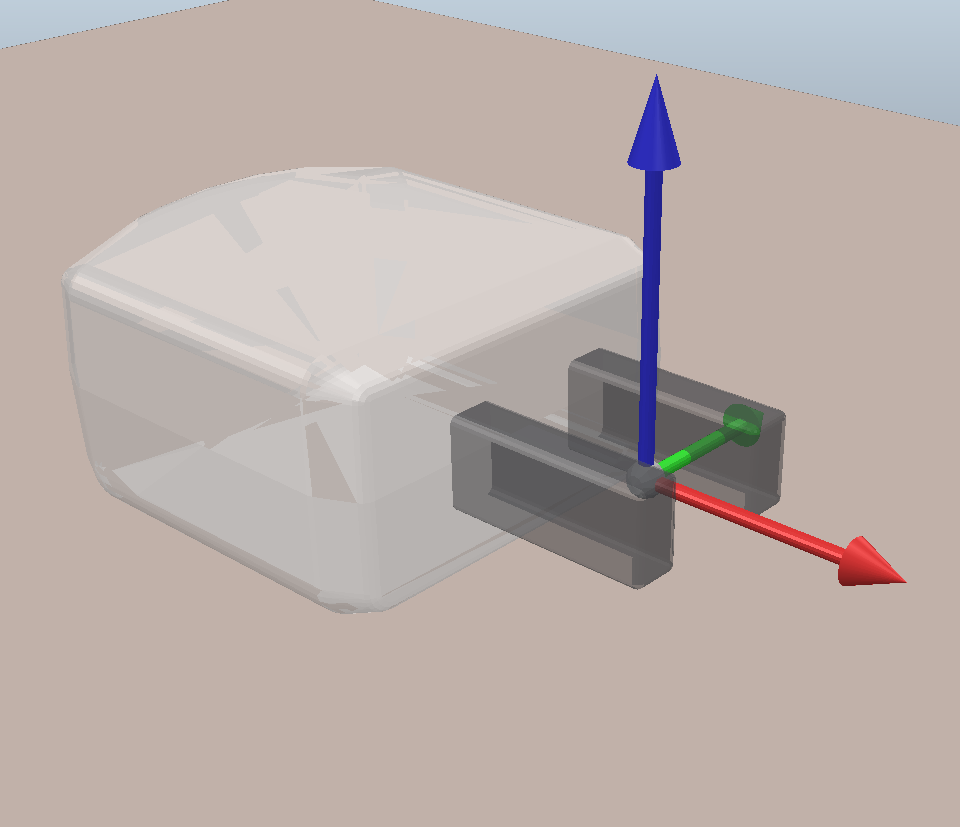
\includegraphics[width=0.5\linewidth]{figures/axis.png}
	\caption[Frame and torque resistance of a Fetch gripper]{The reference frame of a Fetch gripper is shown here. The RGB axis illustrates the maximum static torque on the XYZ axis. A fetch gripper would offer the most static torque on the Z axis and the least static torque on the Y axis.}
	\label{fig:torqueFrame}
\end{figure}

\begin{figure}
	\centering
	\begin{subfigure}[b]{0.4\linewidth}
		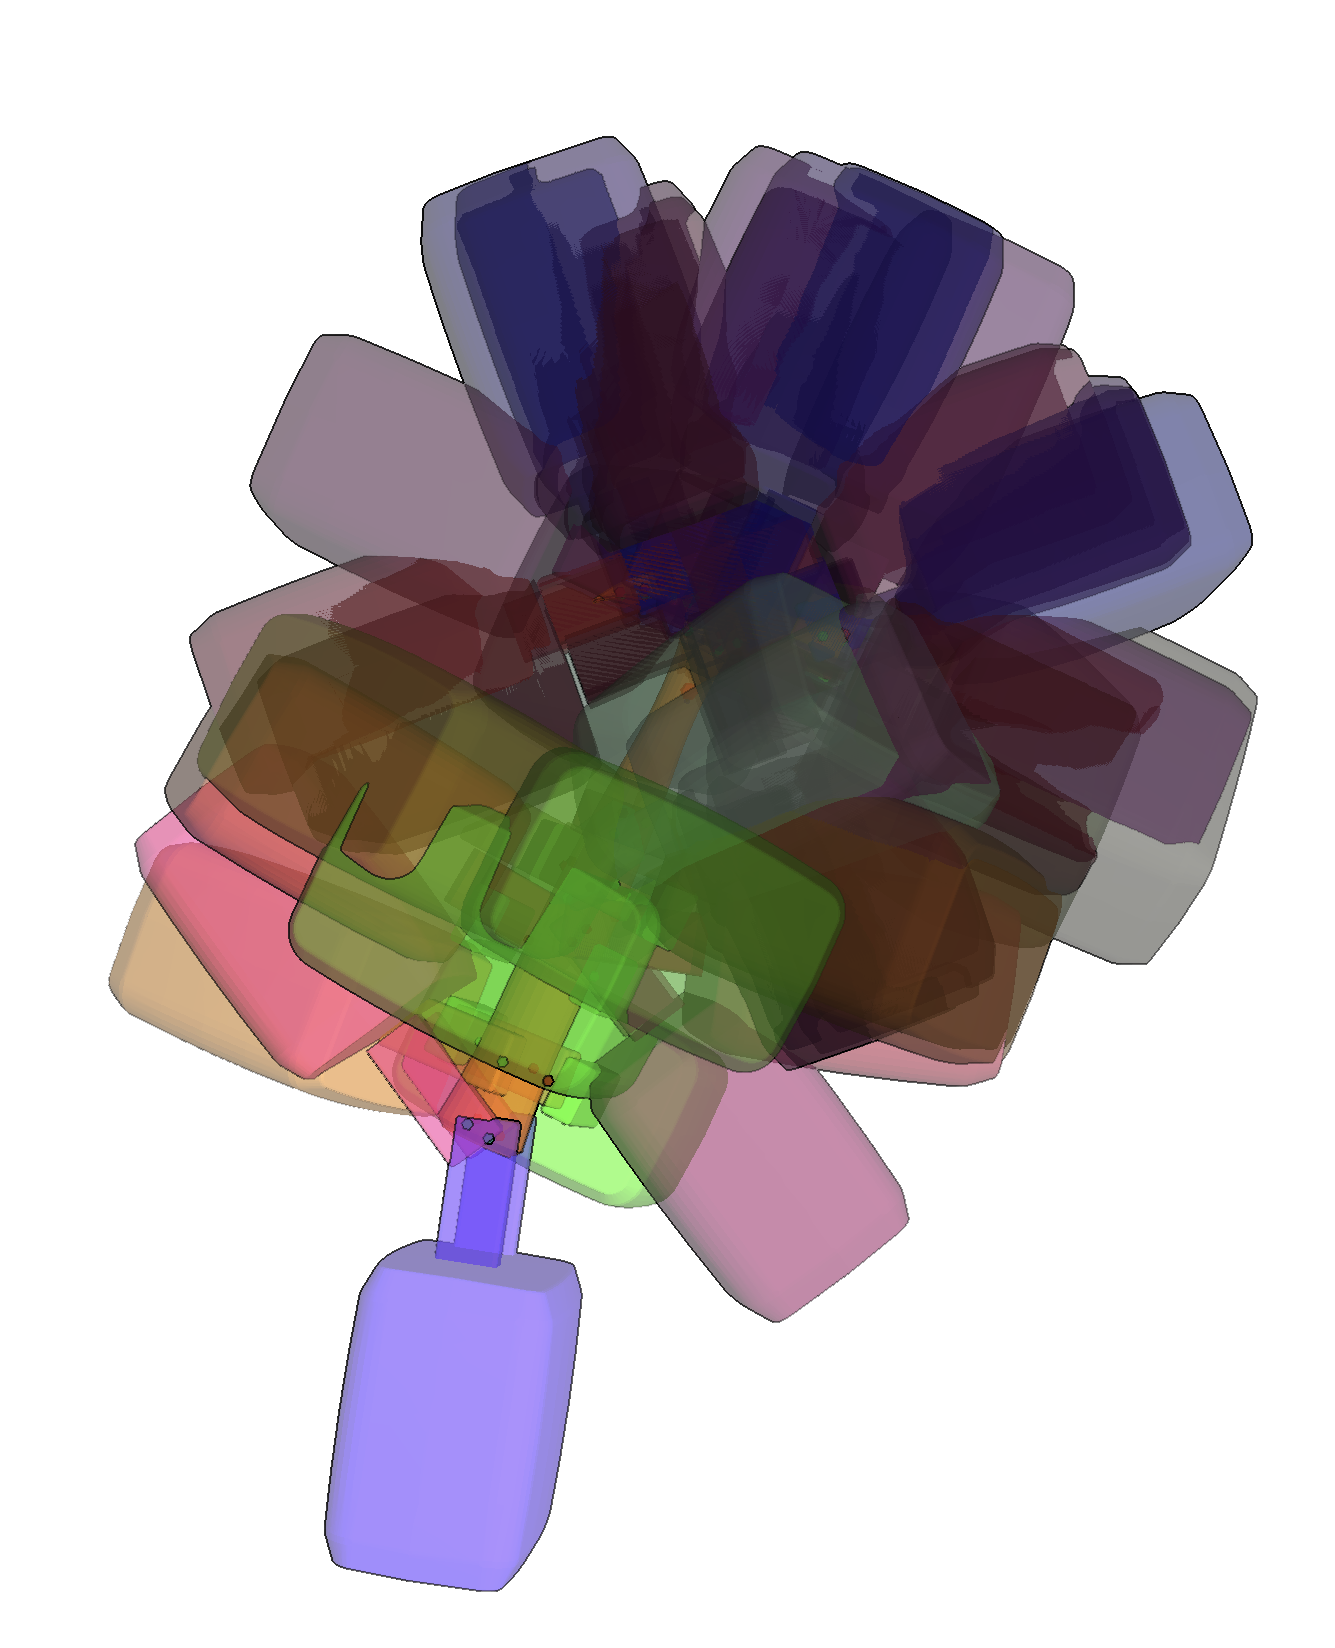
\includegraphics[width=\linewidth]{figures/torques.png}
		\caption{Torques}\label{classificationfiga}
	\end{subfigure}%
	\hfill
	\begin{subfigure}[b]{0.4165\linewidth}
		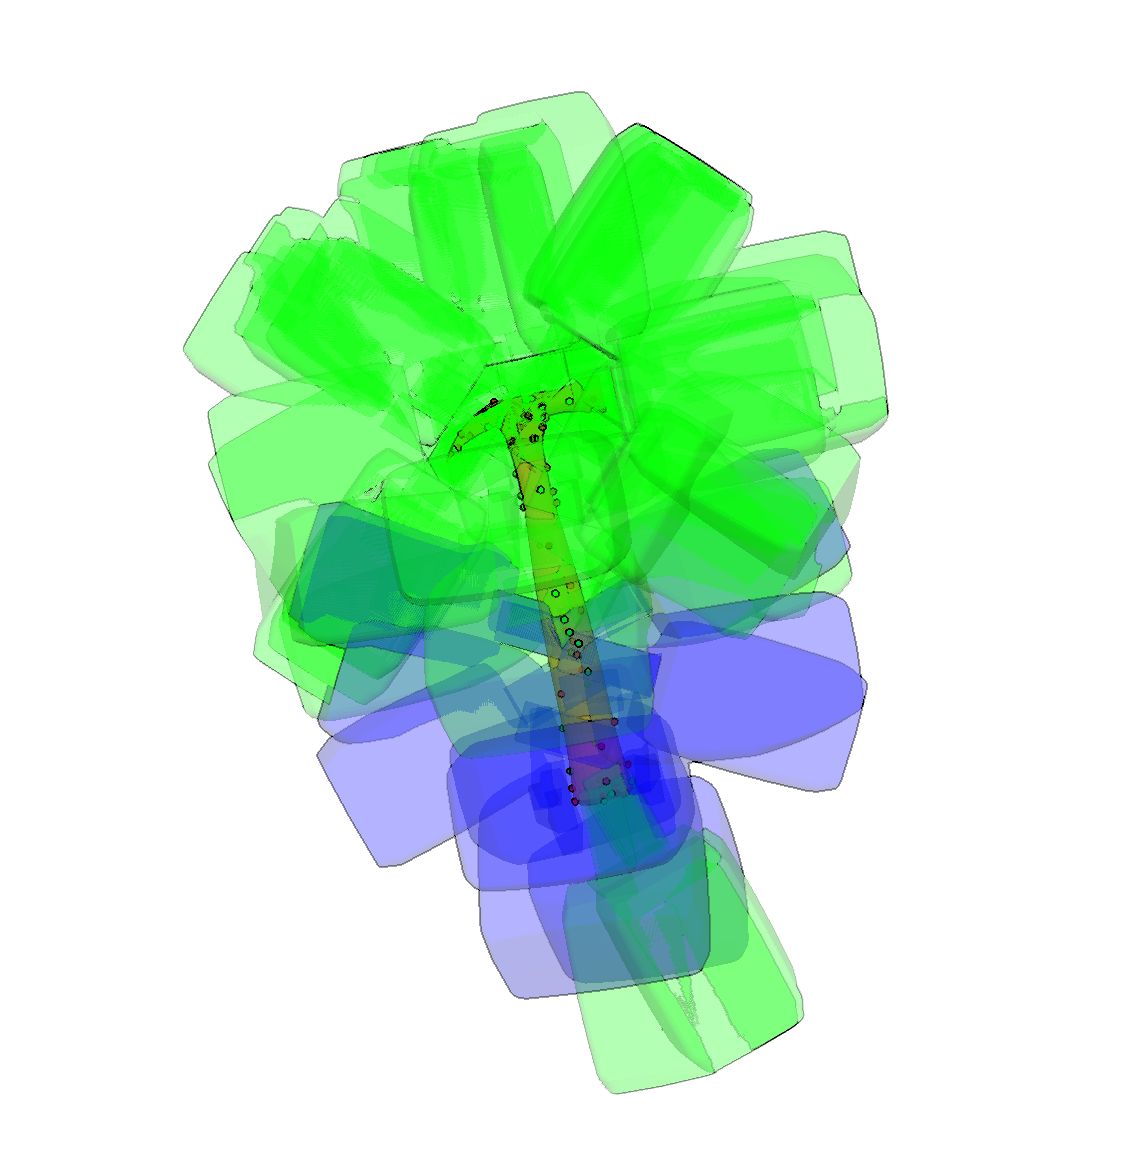
\includegraphics[width=\linewidth]{figures/classified.png}
		\caption{Classifications}\label{classificationfigb}
	\end{subfigure}%
	\caption[Example of torques and the subsquent classifciations made for stable lifting grasp poses]{This example shows the torque analysis and subsequent classification of grasp poses for a hammer object. Each grasp pose is shown as a transparent gripper. (a) shows the torques in gripper XYZ frame. The three torques are visualized as RGB values in each grasp pose. (b) shows the subsequent classification made based on the torques in each axis. The green grasp poses are stable lifting poses while blue ones are not. Notice that two grasp poses at the end of the handle are still classified as stable even though they generate a large torque.}
	\label{fig:classificationExample}
\end{figure}


\chapter{Experiments and Results}
No individual experiments were performed to assess the performance of the stand-alone grasp analyzer. Rather, the grasp analyzer was integrated with a multi-modal planner \cite{iRos2023} to perform pick-and-place tasks both in-simulation and in-real-world experiments. Since both the grasp analyzer and the multi-modal planner has to perform to succeed in a task, the experiments would reflect the performance of the grasp analyzer. 

The robot is asked to pick up an object from a cluttered table in a stable manner. To ensure stability during pickup and placement, the multi-modal planner uses stable sliding grasp poses to relocate the object to a position where a stable lifting pose is feasible; then, the planner uses the stable lifting pose to pick up and place the object.  For each scene and object, a set of trials are performed using the grasp analyzer enabled multi-modal planner and another set of trials are performed using only Contact-GraspNet and an RRT-based planner. The stability of each solution is then compared.

\section{Simulation experiments}
\subsection{Setup}
The simulation experiments are performed in Coppeliasim \cite{coppeliasim} on a simulated Fetch platform. A total of 12 different objects in 12 distinct scenes are performed with the Bullet physics engine. The scene consists of multiple object place on a table, creating a cluttered environment. A Fetch platform, having a parallel gripper with 100 N of grasping force, is positioned at some distance in front of the table. In the first 6 scenes, the target objects are deliberately place in locations where stable lifting poses are initially infeasible. In the remaining 6 scenes, objects are placed randomly.

\subsection{Experiment Trials and Stability Metric}
A trial in the simulation experiment involves the robot grasping the object and then removing the supporting table from the simulation. After the table has been removed fro 5 seconds, a stability core is measured. \emph{Grasping Stability} is measured by the inverse of the object's rotational change relative to the gripper after the table has been removed: $\textrm{stability} = \frac{1}{\Delta R}$. A stable grasp would result in a low object pose change relative to the gripper after grasp, and thus a higher stability score. We also measure the final height of the object after the table has been removed. If the height of the object is less than the height of the removed table, then the object is considered to be dropped. In this case, the stability score is set to 0, indicating a failure. For each object, 10 total trials were run: 5 trials on the Contact-GraspNet and RRT based baseline system and 5 trials on the grasp analyzer and multi-modal task planner based system. The performances of the systems are judged based on the average stability score in a scene.

\subsection{Results}
Results are shown in Table \ref{sim_result}. In all of the scenes, our method achieved on-par or higher stability scores compared to the baseline method. For certain scenes and objects, the baseline was unable to complete the grasping task entirely, resulting in a stability score of 0. In contrast, our grasp analyzer and multi-modal planner were able to identify and execute stable grasps in all of the scenes. This proves that the grasp analyzer's judgments of stable sliding and lifting grasps are sound.

\begin{table}[!h]
	\centering
	\caption[Simulation Experiment Results]{Simulation Experiment Result}
	\label{sim_result}
	\begin{center}
		\begin{tabular}{|c|c|cc|}
			\hline
			\multirow{2}{*}{object name} & \multirow{2}{*}{object mass(kg)} & \multicolumn{2}{c|}{avg. stability (higher is better)}             \\ \cline{3-4} 
			&                              & \multicolumn{1}{c|}{baseline} & our method \\ \hline
			hammer                       & 0.10                          & \multicolumn{1}{c|}{1.04}        & \textbf{9.06}         \\ \hline
			pan                          & 0.16                          & \multicolumn{1}{c|}{1.71}        & \textbf{5.91}         \\ \hline
			candy bar                       & 0.16                          & \multicolumn{1}{c|}{0.00}        & \textbf{32.6}         \\ \hline
			microphone                     & 0.10                          & \multicolumn{1}{c|}{23.5}        & \textbf{41.6}         \\ \hline
			level                      & 0.51                          & \multicolumn{1}{c|}{0.00}        & \textbf{6.23}         \\ \hline
			wrench                           & 0.12                          & \multicolumn{1}{c|}{0.00}        & \textbf{13.5}         \\ \hline
			tissue box                      & 0.80                          & \multicolumn{1}{c|}{3.92}        & \textbf{4.36}         \\ \hline
			cereal                       & 0.12                          & \multicolumn{1}{c|}{5.94}        & \textbf{25.3}         \\ \hline
			can                          & 0.10                          & \multicolumn{1}{c|}{19.3}        & \textbf{68.6}         \\ \hline
			caliper                     & 0.18                          & \multicolumn{1}{c|}{5.06}        & \textbf{8.29}         \\ \hline
			dispenser                     & 0.25                          & \multicolumn{1}{c|}{0.71}        & \textbf{35.9}         \\ \hline
			remote                     & 0.23                          & \multicolumn{1}{c|}{0.35}        & \textbf{5.11}         \\ \hline
			
		\end{tabular}
	\end{center}
\end{table}

\section{Real World Experiments}

\subsection{Setup}

We conducted real-world experiments on three objects - a hammer, a pan, and an espresso machine handle - placed on a cluttered table, as shown in Fig.~\ref{manipulation_objects}. Initially, the hammer and pan were positioned in a pose where achieving high-quality grasps was not feasible, while the espresso machine handle was placed near an obstacle that made high-quality grasps unattainable due to collision. During running the experiment, we tasked the robot with moving those objects into a pre-placed bin using both the baseline method and grasp analyzer and multi-modal planner based method.

\begin{figure}
	\centering
	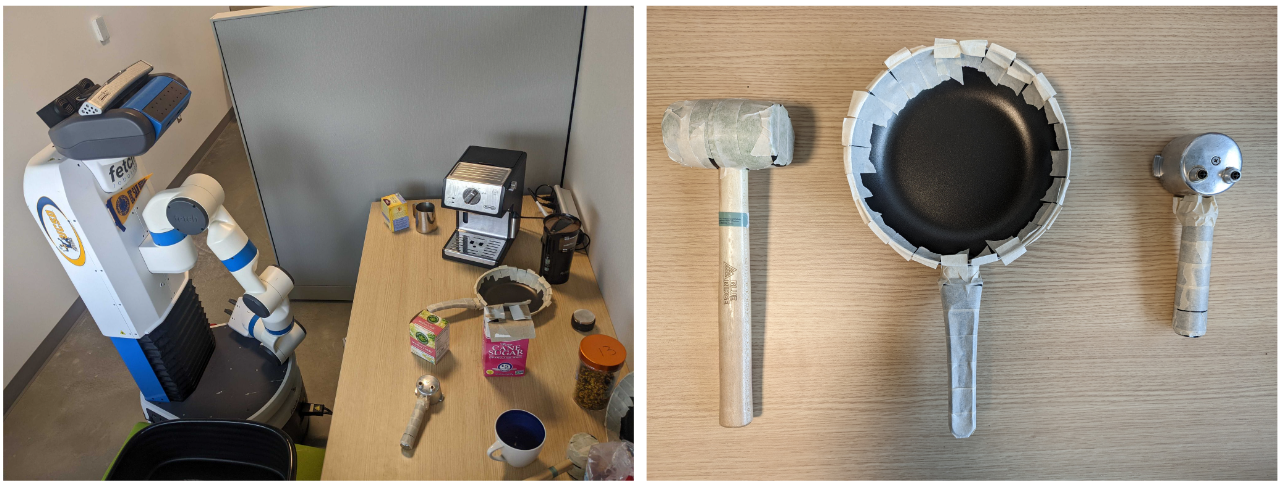
\includegraphics[width=0.9\textwidth]{figures/objects.png}
	\caption{\label{manipulation_objects} Left: the setup of the real-world experiment with Fetch. Right: Objects~(hammer, pan, and espresso machine handle) used in the real-world experiment.}
\end{figure}

\subsection{Results} 
Our multi-modal planner was successful in placing objects into the bin after a few trials. The baseline planner, on the other hand, was unable to successfully place the objects entirely. In the case of the hammer, once the gripper grasped the handle and lifted it up, the gravitational torque caused the hammer to rotate about the contact point and remain in contact with the table \ref{fig:real_world_hammer}. This caused the hammer to drag across the table during placement and ultimately grasp on the hammer failed. With our method, as shown in the lower four figures, our planner determined that the low-quality grasps on the handle were insufficient to lift the hammer, prompting the planner to rearrange the hammer to bring it closer. This adjustment enabled the robot to grasp the hammer in the middle where the predicted center of mass (COM) caused minimal gravitational torque and lift it up successfully.

\begin{figure}
	\centering
	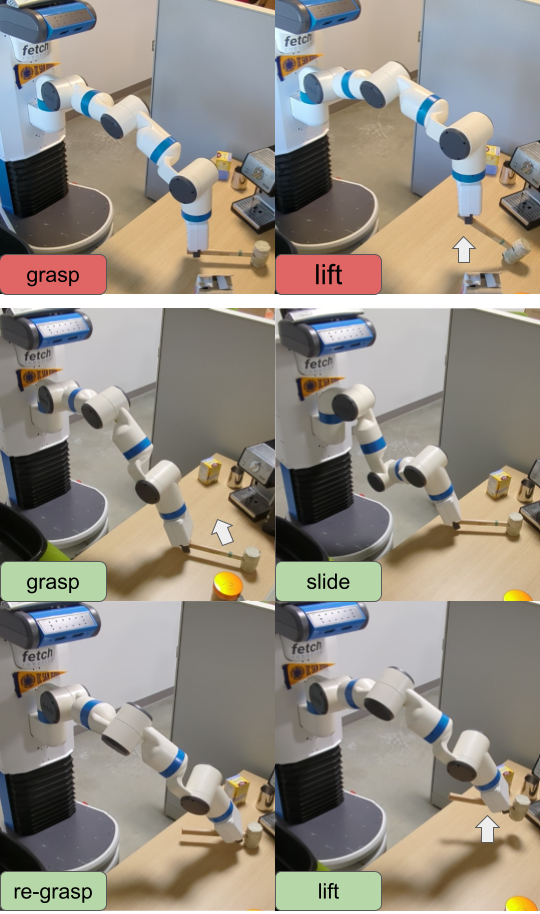
\includegraphics[width=0.7\textwidth]{figures/hammer_real_world.png}
	\caption[Example of an object during real world experiments]{ Upper: Without rearrangement, the hammer rotates around the grasping point during lifting. Lower: With rearrangement, before lifting, the robot identifies stable sliding and lifting grasp and slides the hammer into a better position for reliable lifting.}
	\label{fig:real_world_hammer}
\end{figure}

\chapter{Conclusions and Discussion}
\section{Conclusions}
In this thesis we considered the problem of recommending grasps that enable stable manipulation of objects by a parallel gripper. We created a grasp analyzer that combines learning-based method with physics based methods that can identify stable sliding grasps and stable lifting grasps. The grasp analyzer works on unseen object with arbitrary geometric shapes. This grasp analyzer, combined with a multi-modal planner, was able to complete pick-and-place tasks in a stable manner both in-simulation and in the real world. 

\section{Discussion}
One major weakness of the CoM predictor is objects with highly unevenly-distributed mass. This uneven distribution of mass usually originates from the use of different materials in different parts of the object. Therefore, a viable path for future work would be to add color as a feature onto the partial point cloud of the object. This new feature would allow the model to identify materials and thus predict uneven distribution in mass. This would require careful data generation or input processing as incorrect representation of material colors could lead to poor sim-to-real results.

Another potential direction for future work would be an end-to-end learning-based model that directly identifies stable sliding and lifting grasp poses. This could be achieved with a distillation-like framework \cite{hinton2015distilling}. In such a setup, the output of the current learning-physics hybrid grasp analyzer would be used to generate learning targets for an end-to-end neural network. This could lead to improved efficiency and performance given that the network would directly predict stable sliding and lifting grasp poses.

\appendix

% Stuff at the end of the dissertation goes in the back matter
\backmatter
\bibliographystyle{plain} % Or whatever style you want like plainnat
\bibliography{references}

\end{document}
